% =============================================================================
% report.tex — progress update (work of 16 Nov 2026): conflict-dynamics dashboard and data exploration, the US
% effect over time, UCDP peace agreements, a frozen base specification with one robustness table, full paths with
% permutation inference, a specification curve, a panel VAR and a matched difference-in-differences design.
% Same look as Writing/main.tex and the 9 Nov update.
%
% Build (from this folder):  latexmk -pdf report.tex
% Figures are read directly from the project's results folders (see \graphicspath).
% Bibliography: ../../references.bib (paper) + ../2026-11-09/report_refs.bib + report_refs.bib (new references).
% NUMBERS: runs of 16 Nov 2026 (scripts 13 section 8, 19-22; dashboard build of 16 Nov). Sources of every number:
% empirics/notes/13, 19-22 and dashboard/README.md.
% EXTENDED 17 Nov 2026 (user): score + deaths matching and who-matches-whom (23, fig44), sender groups (24, fig45),
% LP-DiD following the authors' reference code (25, fig47), and a closing assessment (Part D). Numbers: notes 23-25.
% =============================================================================
\documentclass[11pt,a4paper]{article}

\usepackage[T1]{fontenc}
\usepackage[utf8]{inputenc}
\usepackage{lmodern}
\usepackage{microtype}
\usepackage[margin=2.5cm]{geometry}
\usepackage{setspace}
\usepackage{amsmath,amssymb}
\usepackage{graphicx}
\usepackage{booktabs,threeparttable,makecell,tabularx}
\usepackage{caption}
\captionsetup{font=small,labelfont=bf}
\usepackage{float}
\usepackage{enumitem}
\setlist{itemsep=2pt,topsep=4pt}
\usepackage{xcolor}
\usepackage[authoryear,round]{natbib}
\usepackage[colorlinks=true,linkcolor=blue!50!black,citecolor=blue!50!black,urlcolor=blue!50!black]{hyperref}
\usepackage{mdframed}

\graphicspath{{../../../empirics/results/figures/}}

\newcommand{\sig}[1]{\textsuperscript{#1}}
\newcommand{\parttitle}[1]{\vspace{1.2em}\noindent{\Large\bfseries #1}\par\vspace{0.3em}\hrule\vspace{0.6em}}

\title{Do Sanctions Break the Cycle of Violence?\\[4pt]
\normalsize Update 16.11.2026, extended 17.11.2026}
\author{}
\date{}

\begin{document}
\maketitle
\onehalfspacing

% =============================================================================
\begin{mdframed}[linewidth=0.6pt,innerleftmargin=10pt,innerrightmargin=10pt]
\textbf{Summary for the meeting.}
\begin{enumerate}[leftmargin=*]
\item \textbf{Data exploration.} A conflict-dynamics dashboard (UCDP violence, US conflict participation, US sanctions)
  shows how US sanctions sit relative to conflict: in 1989--99 only 46\,\% of conflict country-years were under any US
  sanction, against 62\,\% in 2010--19 and 78\,\% in 2020--23. In the 1990s a new US case was often the first one
  against a conflict; later it was usually an addition to an existing regime.
\item \textbf{The US result, among countries at war.} Deaths fall two to three years after a new US sanction:
  $-0.25$ log points at $h=2$ in the local projection, $-0.29$ in a matched difference-in-differences, $-0.28$ with
  doubly robust weighting. That is roughly a third fewer deaths in that year. There is no pre-trend, and the estimate is
  outside what randomly reshuffled sanctions produce (permutation $p=0.003$).
\item \textbf{Robustness.} Among wars with country fixed effects, all 192 specifications of a specification curve are
  negative and significant. The decline survives controls for peace agreements and is concentrated in sanctions
  imposed with \emph{no} peace process under way.
\item \textbf{Limits.} The effect is short-lived and does not end wars (no effect on war termination). Across all
  countries it is small and fragile. Whether it fades over the decades depends on the design: the local projection is
  flat, the matching estimate falls from about $-0.5$ (1990s sanctions) to about 0 (2010s). Identification is
  selection on observables throughout.
\item \textbf{Added 17.11 (Part C).} Matching on the score \emph{and} on deaths, a figure of who is compared with whom,
  the comparison by sender (any, US, UN, Western rich), and LP-DiD following the authors' own code. All give the same
  sign for US sanctions in wars; none of the new designs is significant, and the LP-DiD shows that the sanctioned wars
  had escalated 3--5 years before the sanction. In the local projection Western rich and UN sanctions are also followed by
  fewer deaths (UN: slower but cumulating), but only the US effect is supported by matching. Overall assessment: Section~\ref{sec:final}.
\end{enumerate}
\end{mdframed}

\begin{table}[H]
\centering\small
\caption{The US effect at $h=2$ across designs: response of $\log(1+\text{deaths per 100k})$ to a new US sanction}
\label{tab:headline}
\begin{threeparttable}
\begin{tabular}{@{}lcc@{}}
\toprule
Design & In conflict in $t-1$ & All state-years \\
\midrule
Local projection, base specification (D11) & $-0.251$\sig{***} (0.062) & $-0.105$\sig{***} (0.039) \\
\quad permutation $p$ (300 reshuffles) & 0.003 & 0.007 \\
Panel VAR(2), bootstrap & --- & $-0.113$\sig{**} (0.050) \\
Doubly robust IPWRA (0/1 shock) & $-0.284$\sig{***} (0.083) & $-0.127$\sig{***} (0.038) \\
Matched difference-in-differences (ATT) & $-0.289$\sig{**} (0.120) & $-0.141$\sig{**} (0.057) \\
\quad bias-adjusted & $-0.426$\sig{**} (0.171) & $-0.160$\sig{**} (0.063) \\
Propensity-score matching (ATT, caliper 0.2 SD) & $-0.268$ (0.284) & $-0.092$ (0.097) \\
\quad score + deaths in $t$ (17.11) & $-0.224$ (0.273) & $-0.097$ (0.067) \\
LP-DiD, authors' code, $y_{t+2}-y_{t-1}$ (17.11) & $-0.228$ (0.218) & $-0.068$ (0.102) \\
\bottomrule
\end{tabular}
\begin{tablenotes}\footnotesize
\item US cases without ICC case 685, UCDP organised violence, shock years 1991--2019. Standard errors clustered by
state (VAR and propensity-score matching: state-cluster bootstrap). Both matching rows: US sanctions after at least two
years without a new US case (Section~\ref{sec:matching}); LP-DiD: none in the three years before and none in
$t+1..t+h$ (Section~\ref{sec:lpdid}). \sig{*}~$p<0.1$, \sig{**}~$p<0.05$, \sig{***}~$p<0.01$.
\end{tablenotes}
\end{threeparttable}
\end{table}

% =============================================================================
\parttitle{Part A --- Data exploration}
% =============================================================================

\section{The conflict-dynamics dashboard}
\label{sec:dashboard}

The dashboard is a descriptive page (plain HTML and Plotly; built by \texttt{dashboard/build\_*.py}) with UCDP
organised violence by type and country 1989--2025, UCDP/PRIO conflicts with the US as a primary or secondary party,
and GSDB US sanction cases. It has a year selector shared by all panels: the countries behind each year's deaths, a
country timeline with the years under US sanctions, a world map, a heatmap of the 40 deadliest countries, and the
tables of US cases and US conflicts. Nothing on it feeds the estimation.

\paragraph{New panel: who the US sanctioned in a year.} For any year 1989--2023 it lists every GSDB case with the US
among the senders that is in force against a country, marked as \emph{new} (the case begins that year),
\emph{ongoing} (with its start year), \emph{joined} (an existing case extended to the country) or \emph{lifted}
(first year without it), with its type, objective, co-senders and the country's deaths that year. The set matches the
panel's ``US sanction in force'' exactly in every year. Two examples: in 1994 the US had sanctions in force against
52 countries (83 case-targets) and began 7 new cases against 6 countries (among them Haiti, Nigeria and Indonesia);
in 2005, counting the ICC case 685, 139 countries were under a US sanction but only one new case began (Nepal).

\begin{table}[H]
\centering\small
\caption{US sanctions and US conflict participation, by period (dashboard)}
\label{tab:dashboard}
\begin{tabular}{@{}lccc@{}}
\toprule
Period & \makecell{Conflict country-years under\\a US sanction in force} & \makecell{Conflict deaths under\\a US sanction in force} & \makecell{Conflict-years with\\the US as a party} \\
\midrule
1989--99 & 46\,\% & 31\,\% (61\,\% without Rwanda 1994) & 3 \\
2000--09 & 62\,\% & 54\,\% & 25 \\
2010--19 & 62\,\% & 85\,\% & 64 \\
2020--23 & 78\,\% & 94\,\% & 45 (to 2025) \\
\bottomrule
\end{tabular}
\end{table}

\paragraph{What it shows.}
\begin{itemize}[leftmargin=*]
\item In the 1990s US cases often hit conflicts with no US sanction yet; later almost every deadly conflict already
  had one, so a new case is an increment. This fits a larger 1990s effect but is a reading, not a test.
\item The US itself was a party to only 3 conflict-years in 1989--99 (Panama, Gulf War, Kosovo) and to 64 in
  2010--19. The kind of conflicts the US sanctions changed.
\item Bosnia illustrates the counting rules: the 1991 US arms embargo (case 422) is dated to Yugoslavia, so Bosnia
  shows a US sanction in force 1992--96 but no new US case; UCDP never codes the US as a party there.
\end{itemize}

\section{New data}

\begin{itemize}[leftmargin=*]
\item \textbf{UCDP peace agreements and conflict terminations}
  \citep{ucdppeace2022,kreutz2010}: 374 agreements 1975--2021 and 505 ended conflict episodes, located by the
  conflict's country and cleaned to state-years. Agreements peak in the 1990s (166 in 1989--99, 100 in 2000--09, 78 in
  2010--21), so a settlement story for the 1990s US effect was worth testing (Section~\ref{sec:peace}).
\item \textbf{Conflict forecasts} (advisor's suggestion): the Hegre et al.\ forecasting model and the VIEWS archived
  forecasts are downloaded and cleaned to state-years, but not yet used. Published ex-ante forecasts exist for
  2010--2019 (Hegre et al.\ 2013) and from 2022 (VIEWS).
\end{itemize}

% =============================================================================
\parttitle{Part B --- The effect of US sanctions}
% =============================================================================

\section{Base specification}
\label{sec:base}

All US results now use one fixed base specification (decision D11). Every check changes exactly one thing against it.
\begin{equation}
y_{i,t+h} = \beta_h\, x_{it} + \sum_{k=1}^{2}\big(a_{hk}\, y_{i,t-k} + b_{hk}\, x_{i,t-k}\big) + c_h\, y_{it}
+ \alpha_i + \delta_t + \varepsilon_{i,t+h},
\label{eq:lp}
\end{equation}
with $y=\log(1+\text{UCDP deaths per 100k})$, $x$ the number of new US cases without the ICC case 685, state and
year fixed effects, no further controls, standard errors clustered by state, shock years 1991--2019. Controlling for
$y_{it}$ (``shock second'') means a sanction cannot affect deaths in its own year. Outcomes: $y_{t+2}$ and the
cumulative $\sum_{j=0}^{3}y_{t+j}$. Two samples: all state-years, and state-years in conflict in $t-1$ (at least 25
deaths).

\section{Is the US effect a 1990s effect?}
\label{sec:time}

\begin{table}[H]
\centering\small
\caption{US effect by period of the sanction, $h=2$}
\label{tab:periods}
\begin{threeparttable}
\begin{tabular}{@{}lccc@{}}
\toprule
& 1991--99 & 2000--19 & $p$ (equal) \\
\midrule
All state-years & $-0.213$\sig{**} (0.082) & $-0.046$ (0.034) & 0.055 \\
In conflict in $t-1$ & $-0.252$\sig{**} (0.114) & $-0.250$\sig{***} (0.081) & 0.99 \\
\bottomrule
\end{tabular}
\begin{tablenotes}\footnotesize
\item Separate coefficients for shocks before and from 2000 in one regression. With three periods (all state-years):
1991--99 vs.\ 2010--19 $p=0.05$, 1991--99 vs.\ 2000--09 $p=0.27$.
\end{tablenotes}
\end{threeparttable}
\end{table}

Across all state-years the effect sits in the 1990s; among countries at war the local projection finds the same
effect for shocks before and after 2000. Rolling nine-year windows (Figure~\ref{fig:rolling}) show the same contrast.
None of the observable features of US sanctions that changed over time explains the all-state-years gap: arms
embargoes fell from 24\,\% to 3\,\% of new US cases, and the shares of first-time sanctions, UN-backed cases and
conflict objectives moved too, but allowing each its own effect leaves the before/after-2000 gap at $-0.16$ to
$-0.20$. A panel VAR gives the same point estimates as the local projection in every period (e.g.\ all years $-0.113$
vs.\ $-0.105$; 2010--19 $-0.04$ vs.\ $-0.07$) and is not more precise at $h=2$, as expected: up to the lag length both
use essentially the same coefficients.

\begin{figure}[H]
\centering
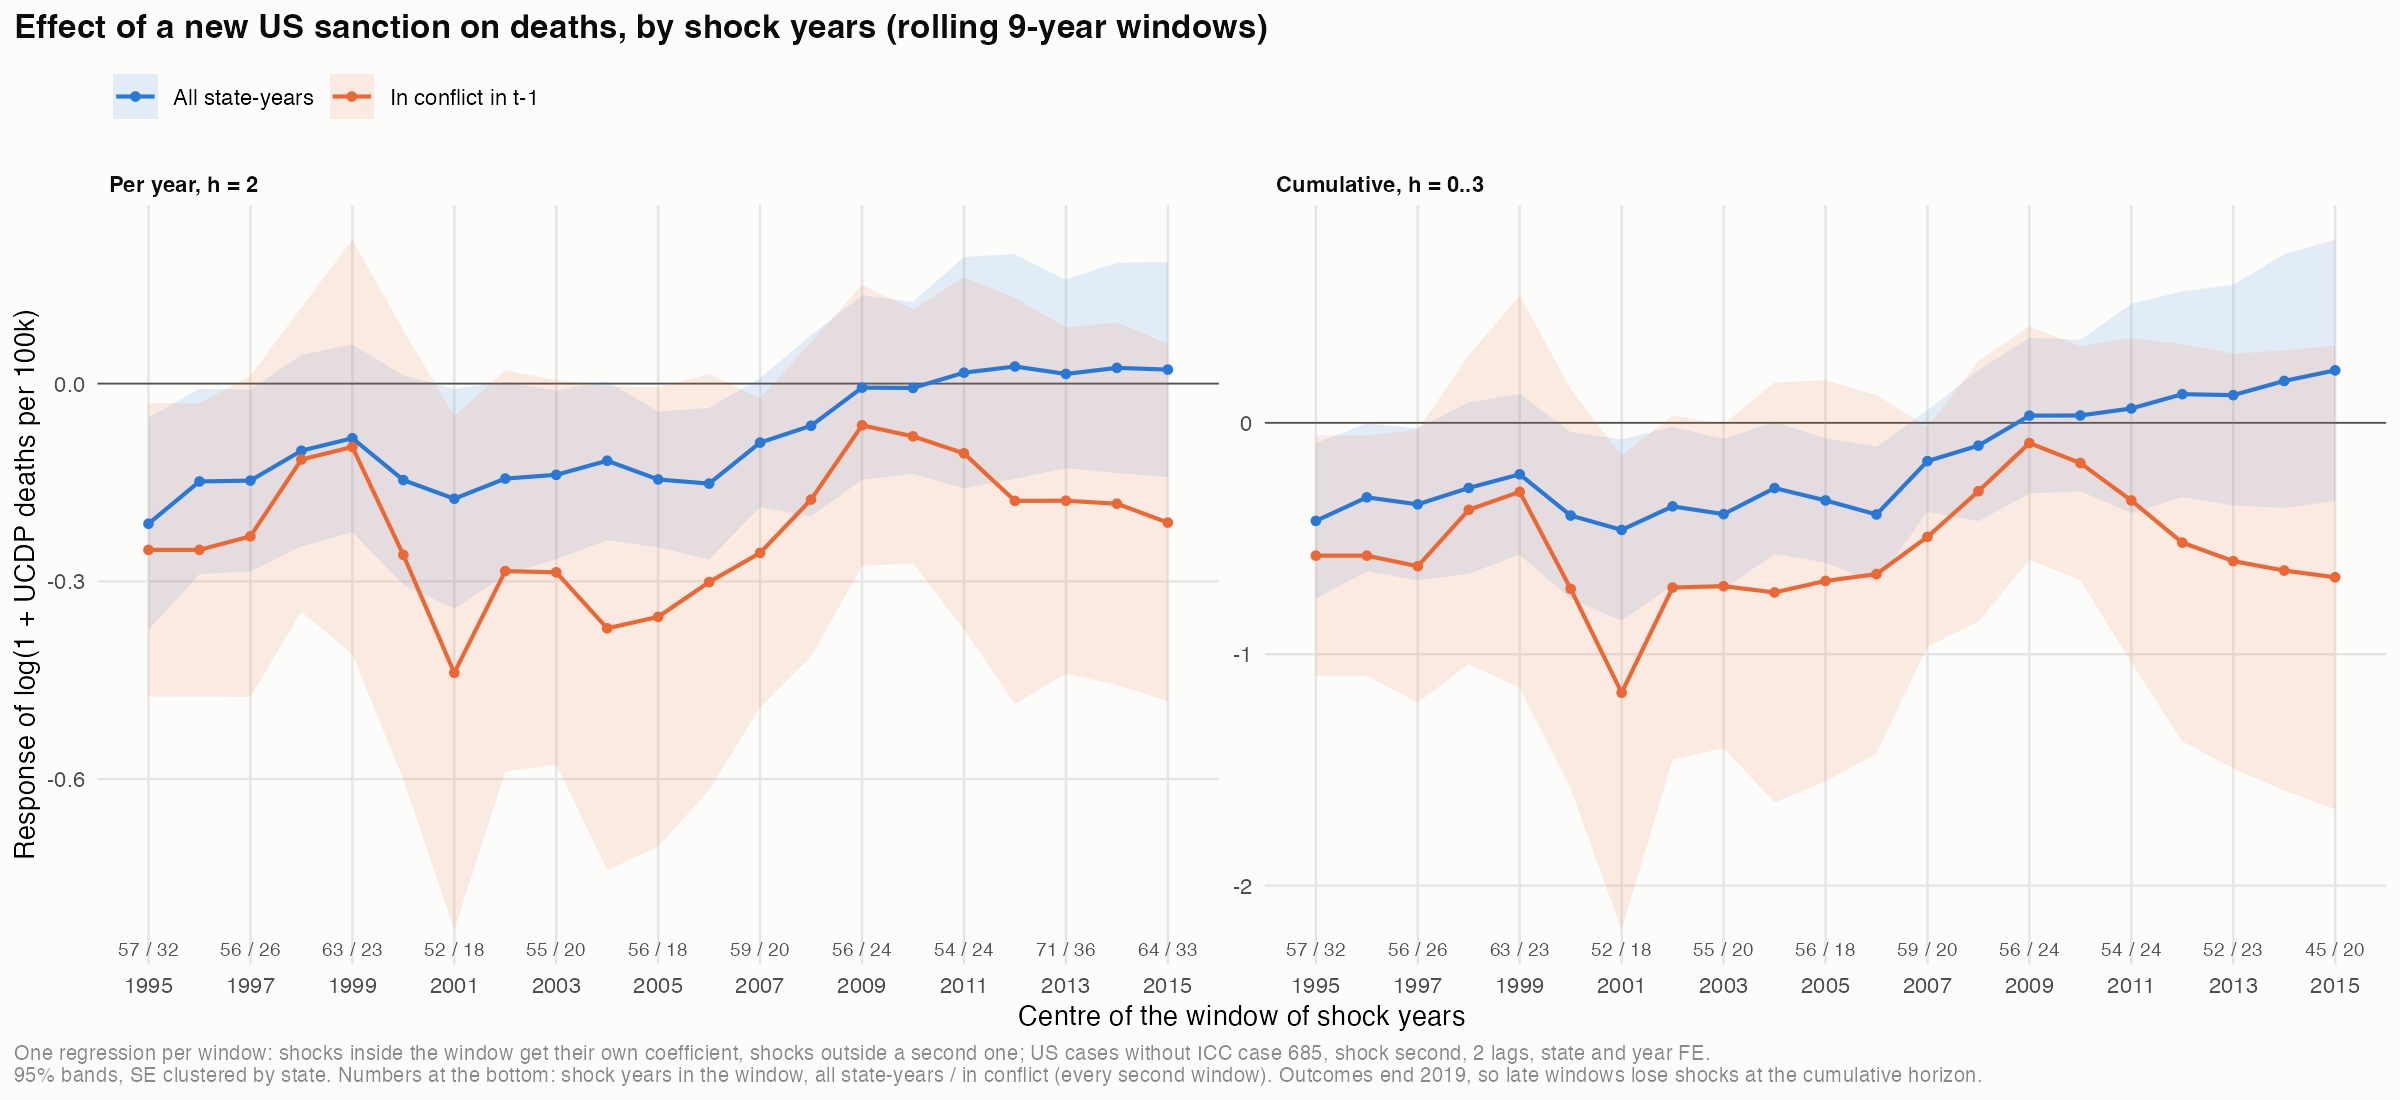
\includegraphics[width=0.95\textwidth]{fig34_lp_us_beta_over_time.png}
\caption{Effect of a new US sanction by the years in which it was imposed (rolling nine-year windows).}
\label{fig:rolling}
\end{figure}

\section{Peace agreements}
\label{sec:peace}

If the US sanctions wars that are already being settled, the decline after sanctions would reflect the settlement.
The data do not support this:
\begin{itemize}[leftmargin=*]
\item Few US sanctions come near an agreement: an agreement in the target in $t-2..t$ for 19\,\% (1990s), 12\,\% and
  9\,\% of US shock-years.
\item Agreement controls (for $t-2..t-1$, up to $t+1$) leave the estimate unchanged: $-0.25$ to $-0.27$ in wars.
\item Splitting the shock: US sanctions imposed with \emph{no} agreement under way $-0.342$\sig{***} (67 shock-years)
  vs.\ with one $-0.050$ (18), $p(\text{equal})=0.10$.
\item US sanctions do not change the probability that a war ends within $t..t+2$ ($+0.022$, mean 0.34), whether by
  agreement, victory or low activity. An agreement in year $t$ makes a new US case \emph{less} likely ($-0.079$\sig{***},
  mean 0.097).
\end{itemize}

\begin{figure}[H]
\centering
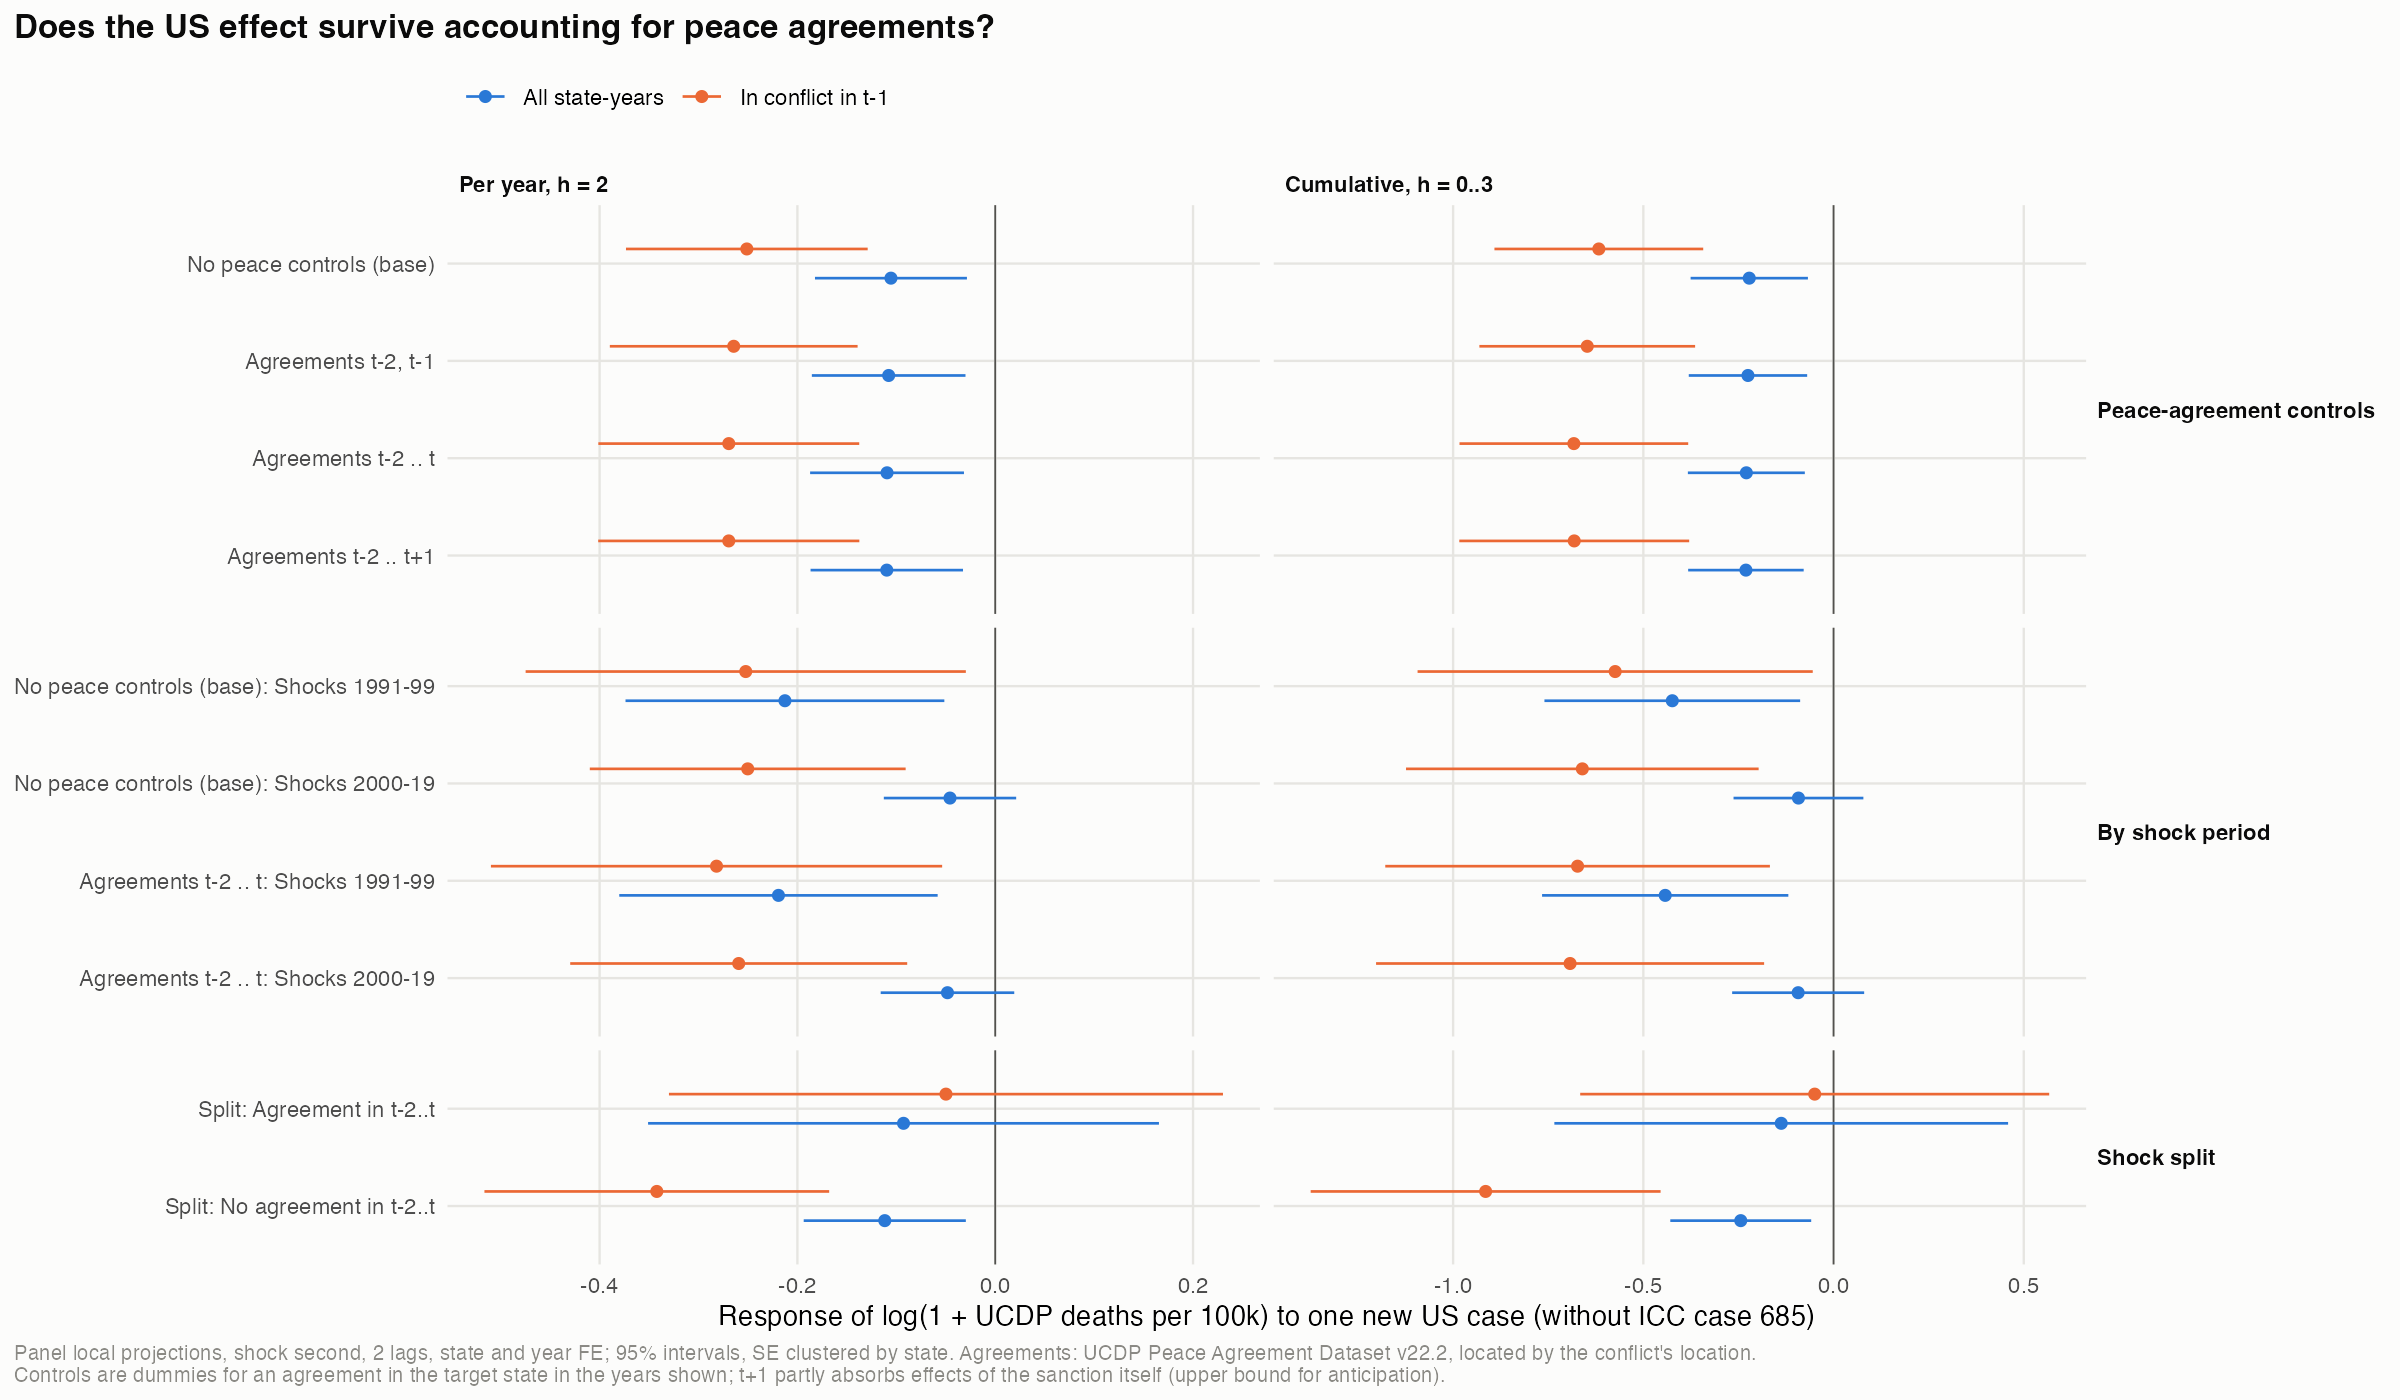
\includegraphics[width=0.85\textwidth]{fig36_peace_process_lp.png}
\caption{The US effect with peace-agreement controls, by period, and split by whether a peace process was under way.}
\end{figure}

\section{One robustness table}

\begin{figure}[H]
\centering
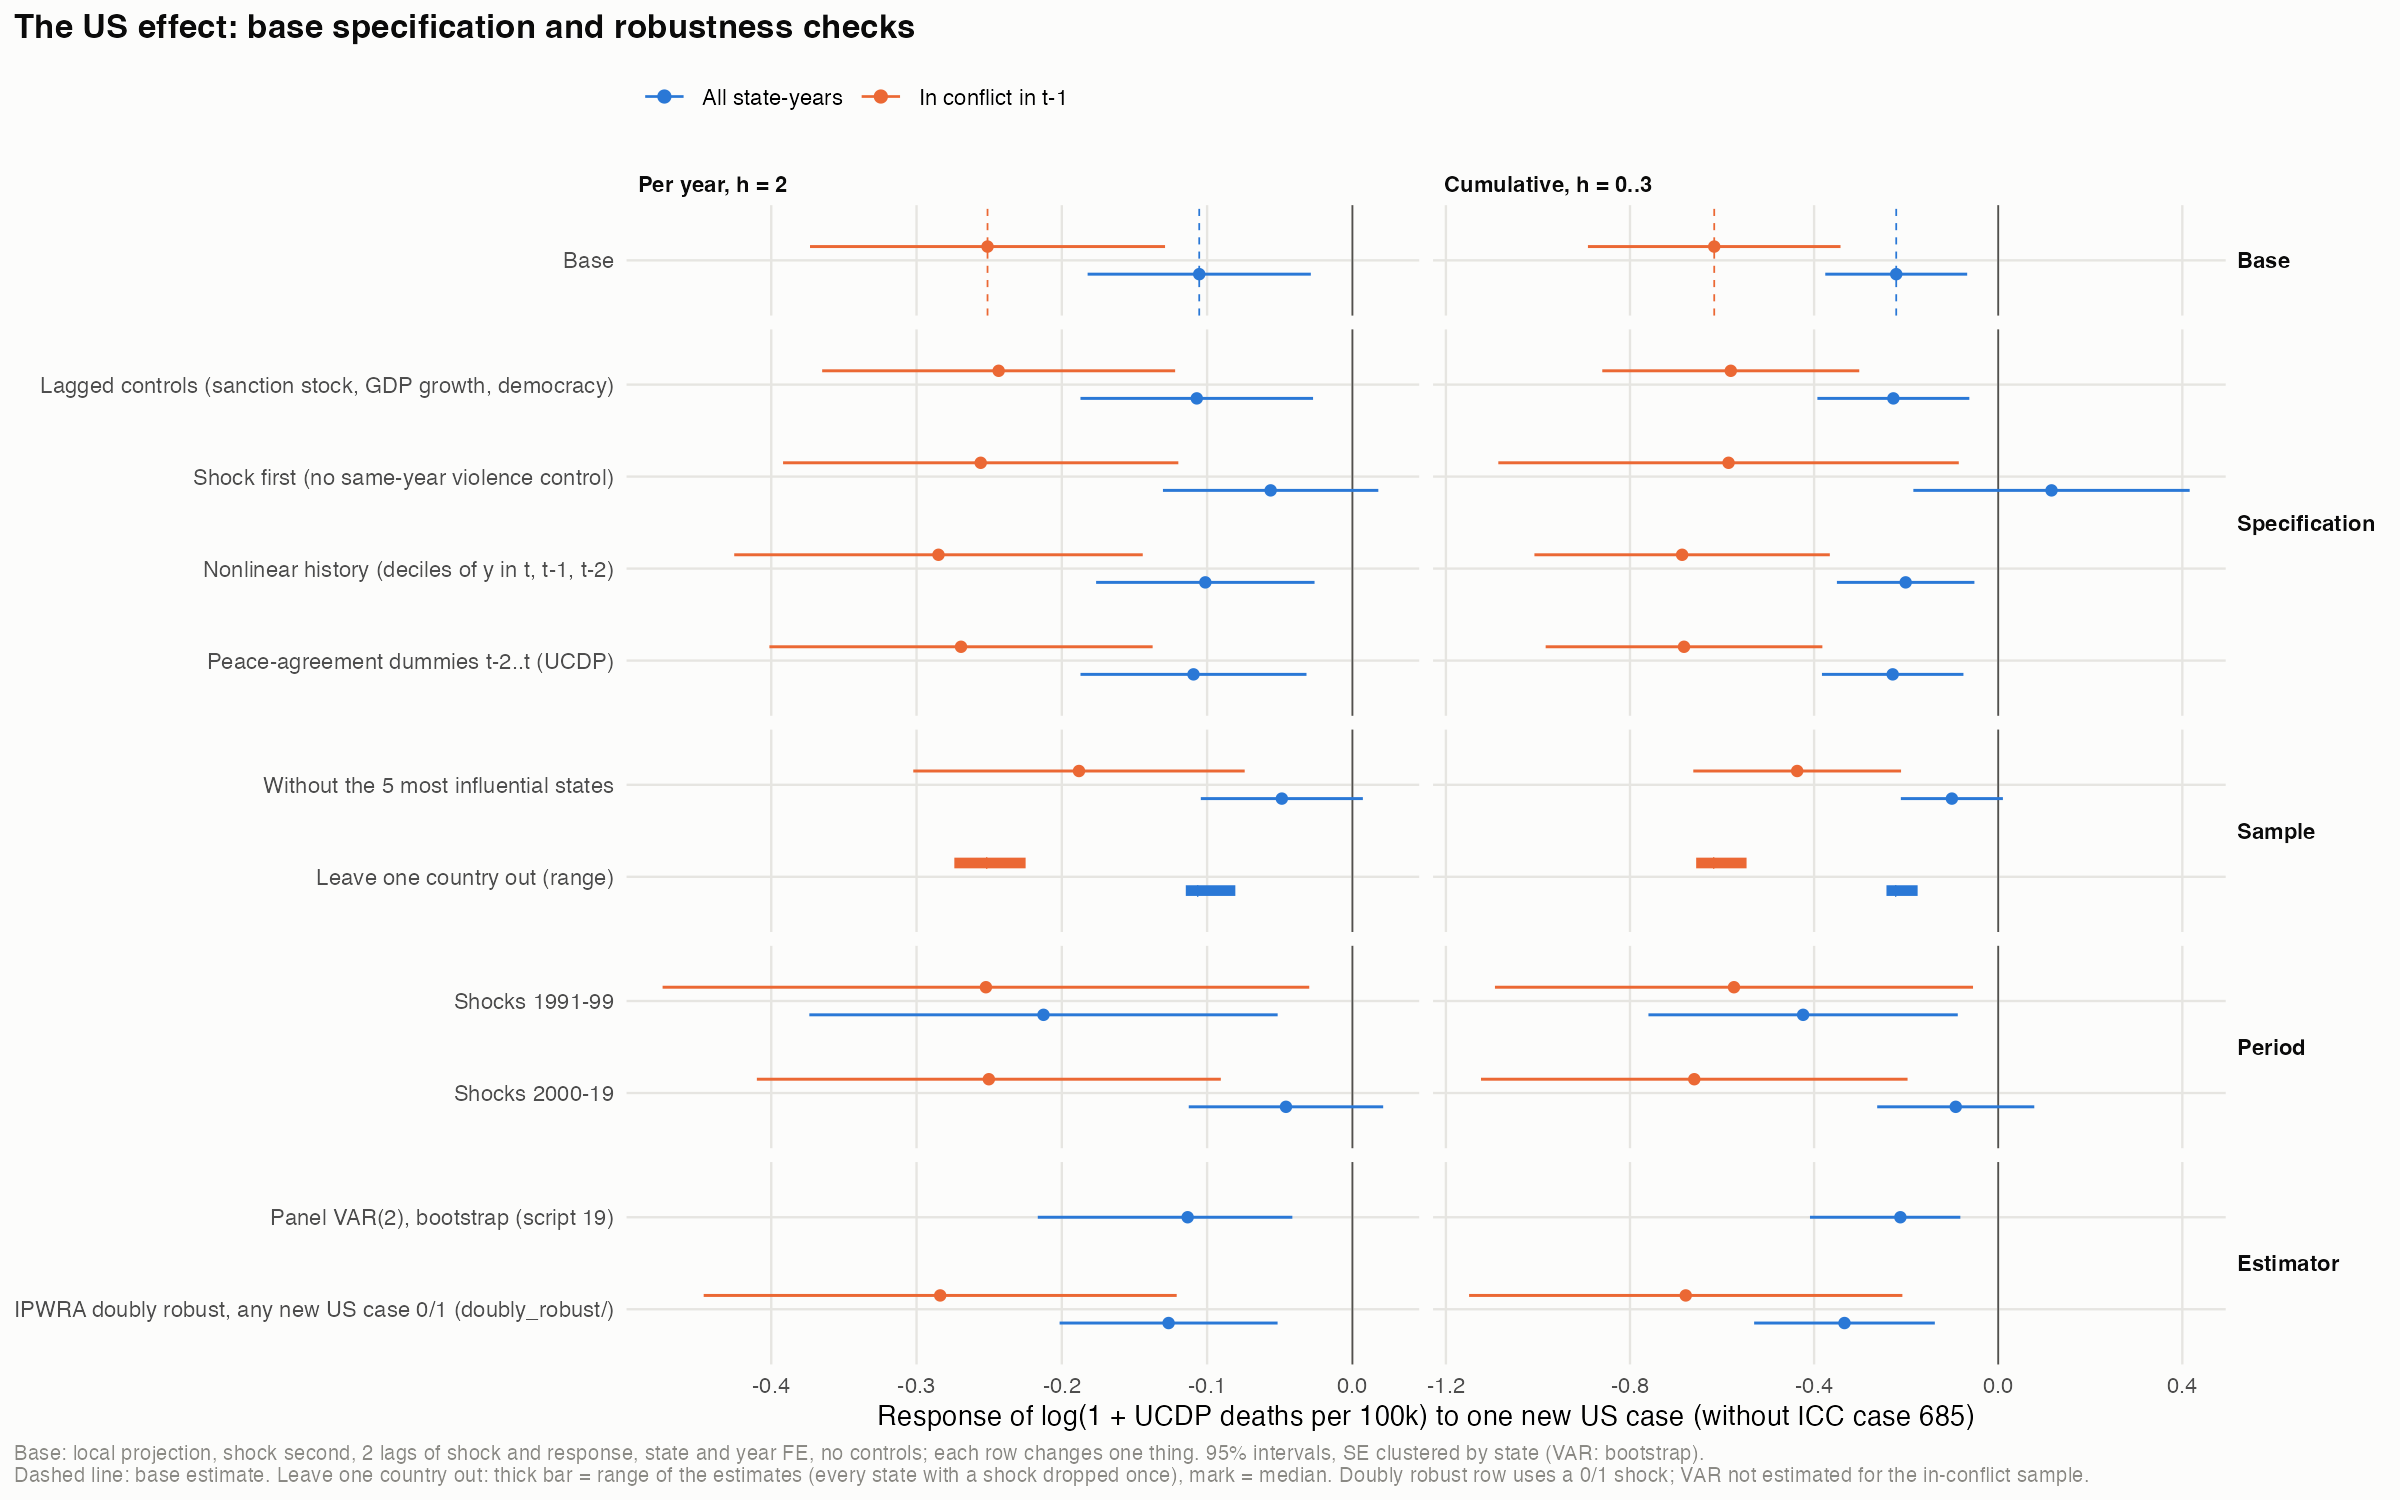
\includegraphics[width=0.9\textwidth]{fig37_us_robustness.png}
\caption{Base specification and one-at-a-time checks. Dashed line: base estimate.}
\label{fig:robustness}
\end{figure}

Among wars every check is negative and significant ($-0.19$ to $-0.29$ at $h=2$), including the two designed to hurt:
dropping the five most influential states (Yugoslavia, Iraq, Nepal, Angola, Liberia) and allowing a same-year
effect. Across all state-years three checks remove the effect: dropping those five states, restricting to shocks
from 2000, and ``shock first'' timing. The last mixes in reverse causality, since violence also triggers sanctions
within the year.

\section{The whole path, and is it noise?}

\begin{figure}[H]
\centering
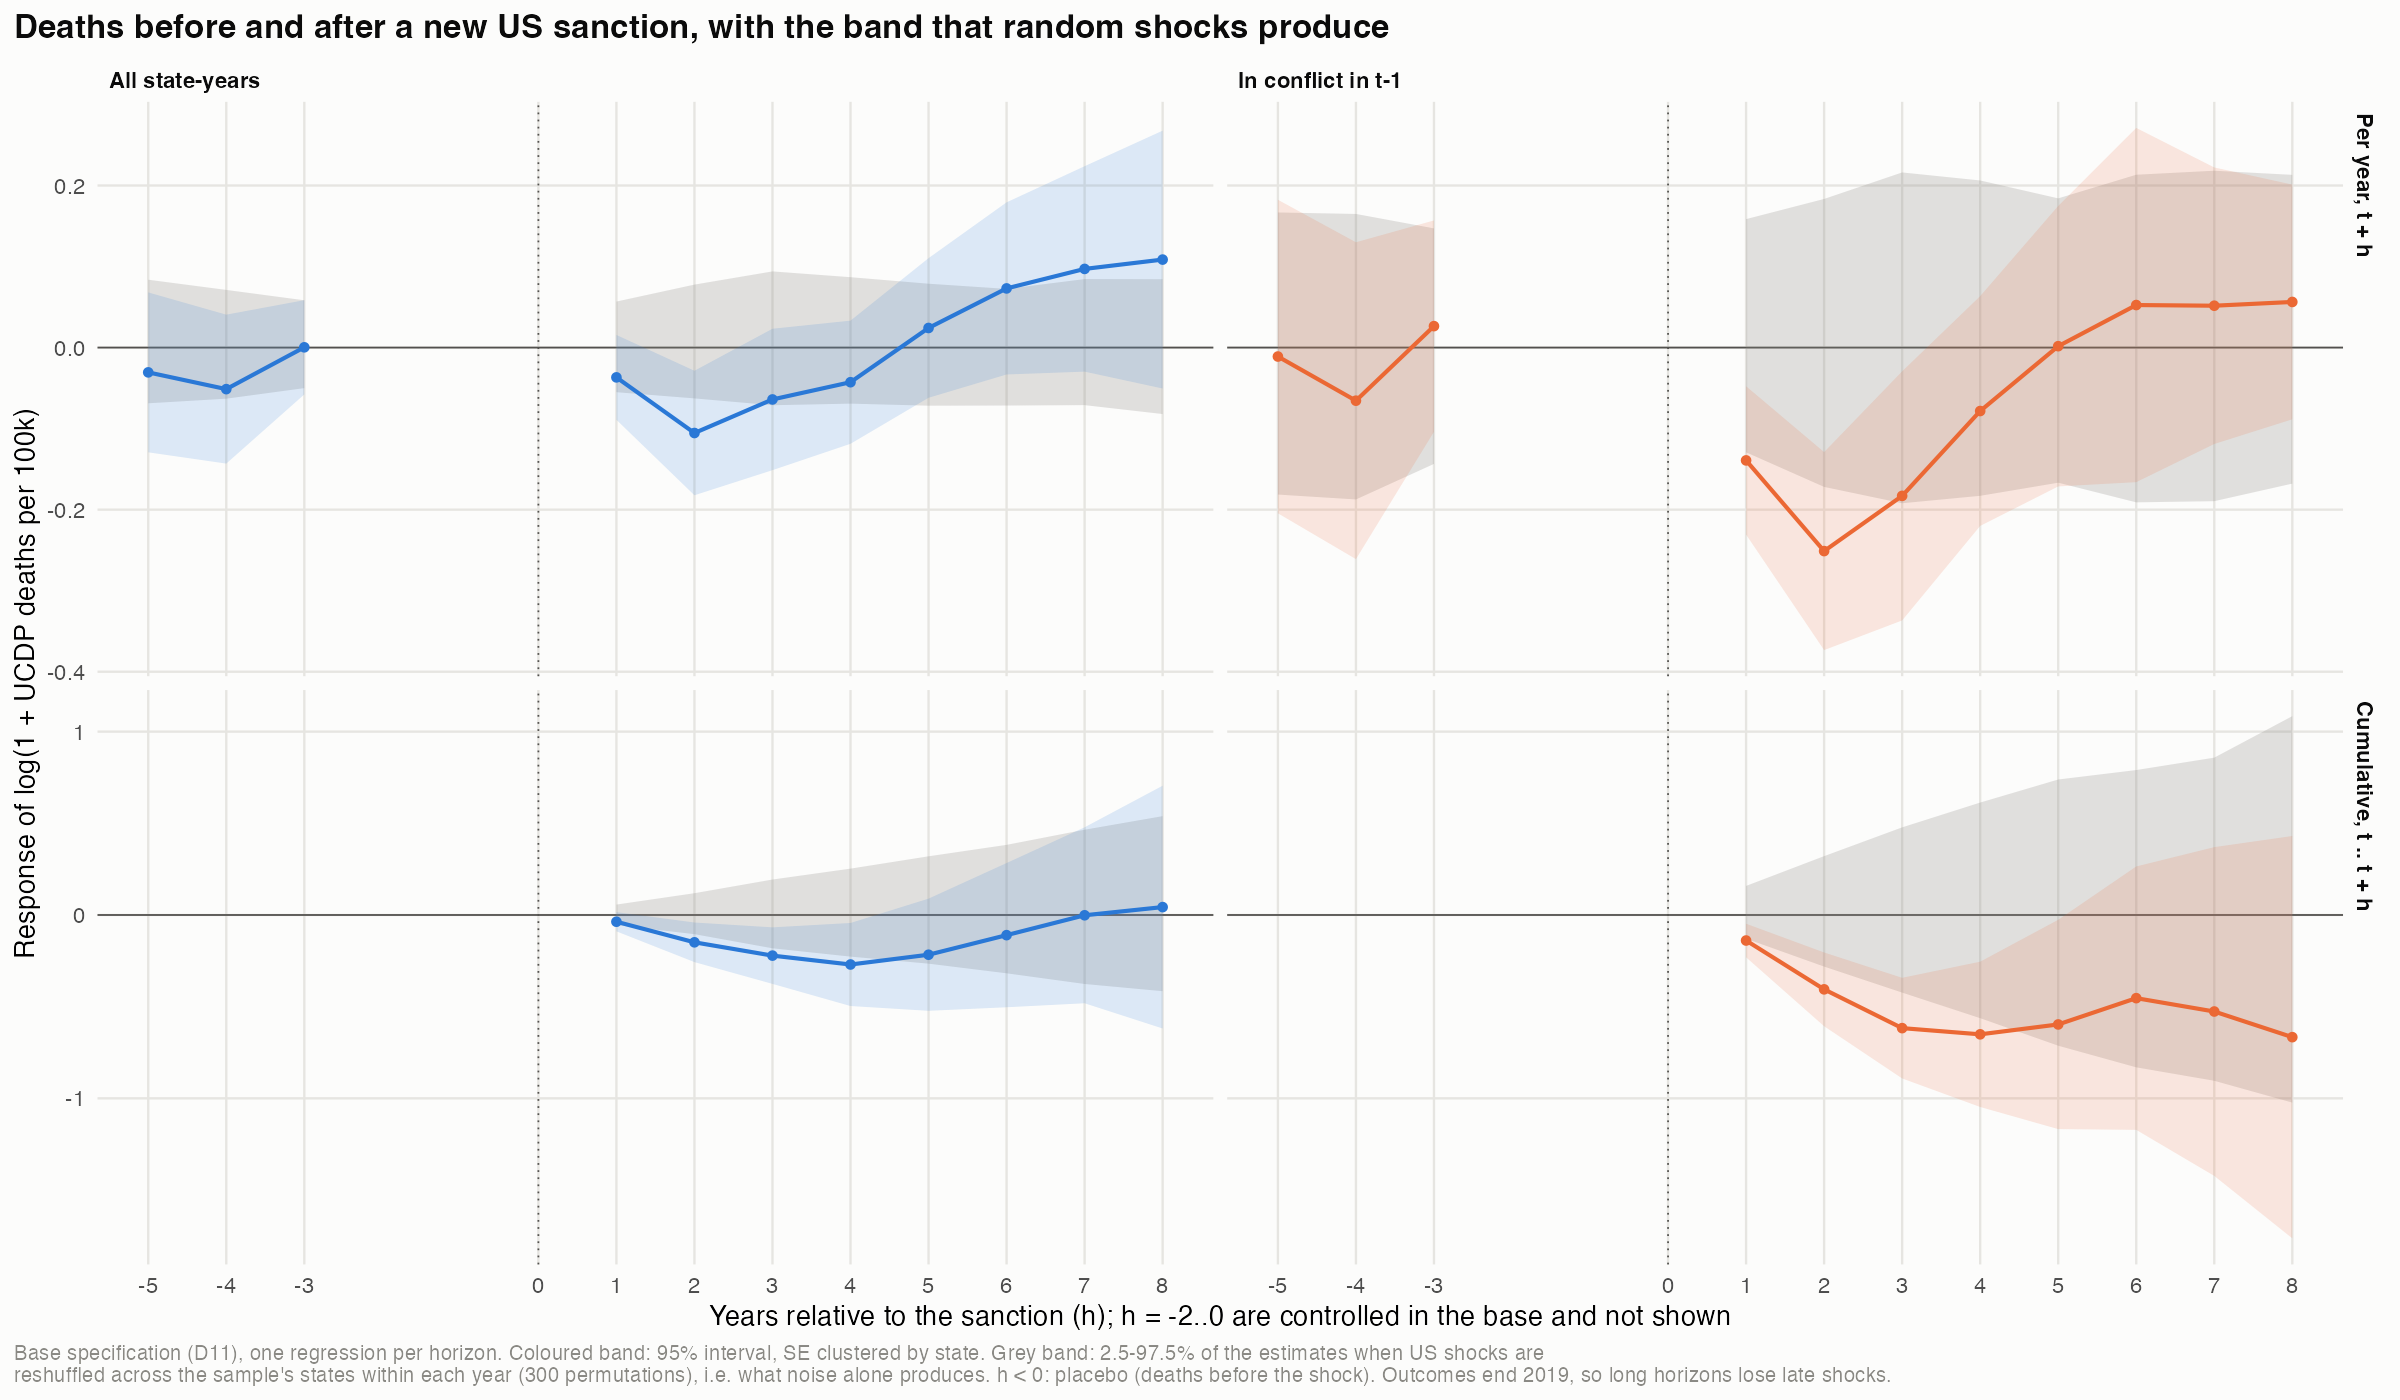
\includegraphics[width=0.95\textwidth]{fig38_us_paths.png}
\caption{Deaths before and after a new US sanction. Grey band: 95\,\% of the estimates when US sanctions are
reshuffled across the sample's countries within each year (300 draws), i.e.\ what noise alone produces.}
\label{fig:paths}
\end{figure}

\begin{itemize}[leftmargin=*]
\item \textbf{No pre-trend:} deaths 3--5 years before a US sanction do not differ.
\item \textbf{Not noise:} among wars the $h=2$ estimate is larger than in all but 0.3\,\% of the reshuffles; corrected
  for looking at six horizons, the family-wise $p$ stays below 0.05 in both samples. The noise band is wider than the
  clustered interval (in wars $\pm0.18$ vs.\ $\pm0.12$), so the permutation $p$-values are the ones to quote.
\item \textbf{A temporary dip:} in wars $-0.14$ ($h=1$), $-0.25$ ($h=2$), $-0.18$ ($h=3$), about zero from $h=5$.
  Across all state-years the dip is followed by positive estimates at $h=6$--8.
\item \textbf{Size:} for the median war year (1.18 deaths per 100k), $-0.25$ means about 0.70 per 100k two years
  later, roughly 40\,\% fewer deaths in that year; for a country of 20 million, about 236 deaths down to 140.
\end{itemize}

\section{Specification curve}

All combinations of sample, timing, lag length (1--3), fixed effects (state or region, with year), lagged controls,
linear or decile history, peace-agreement dummies, the five influential states, and count or 0/1 coding: 768
specifications per outcome \citep{simonsohn2020}.

\begin{figure}[H]
\centering
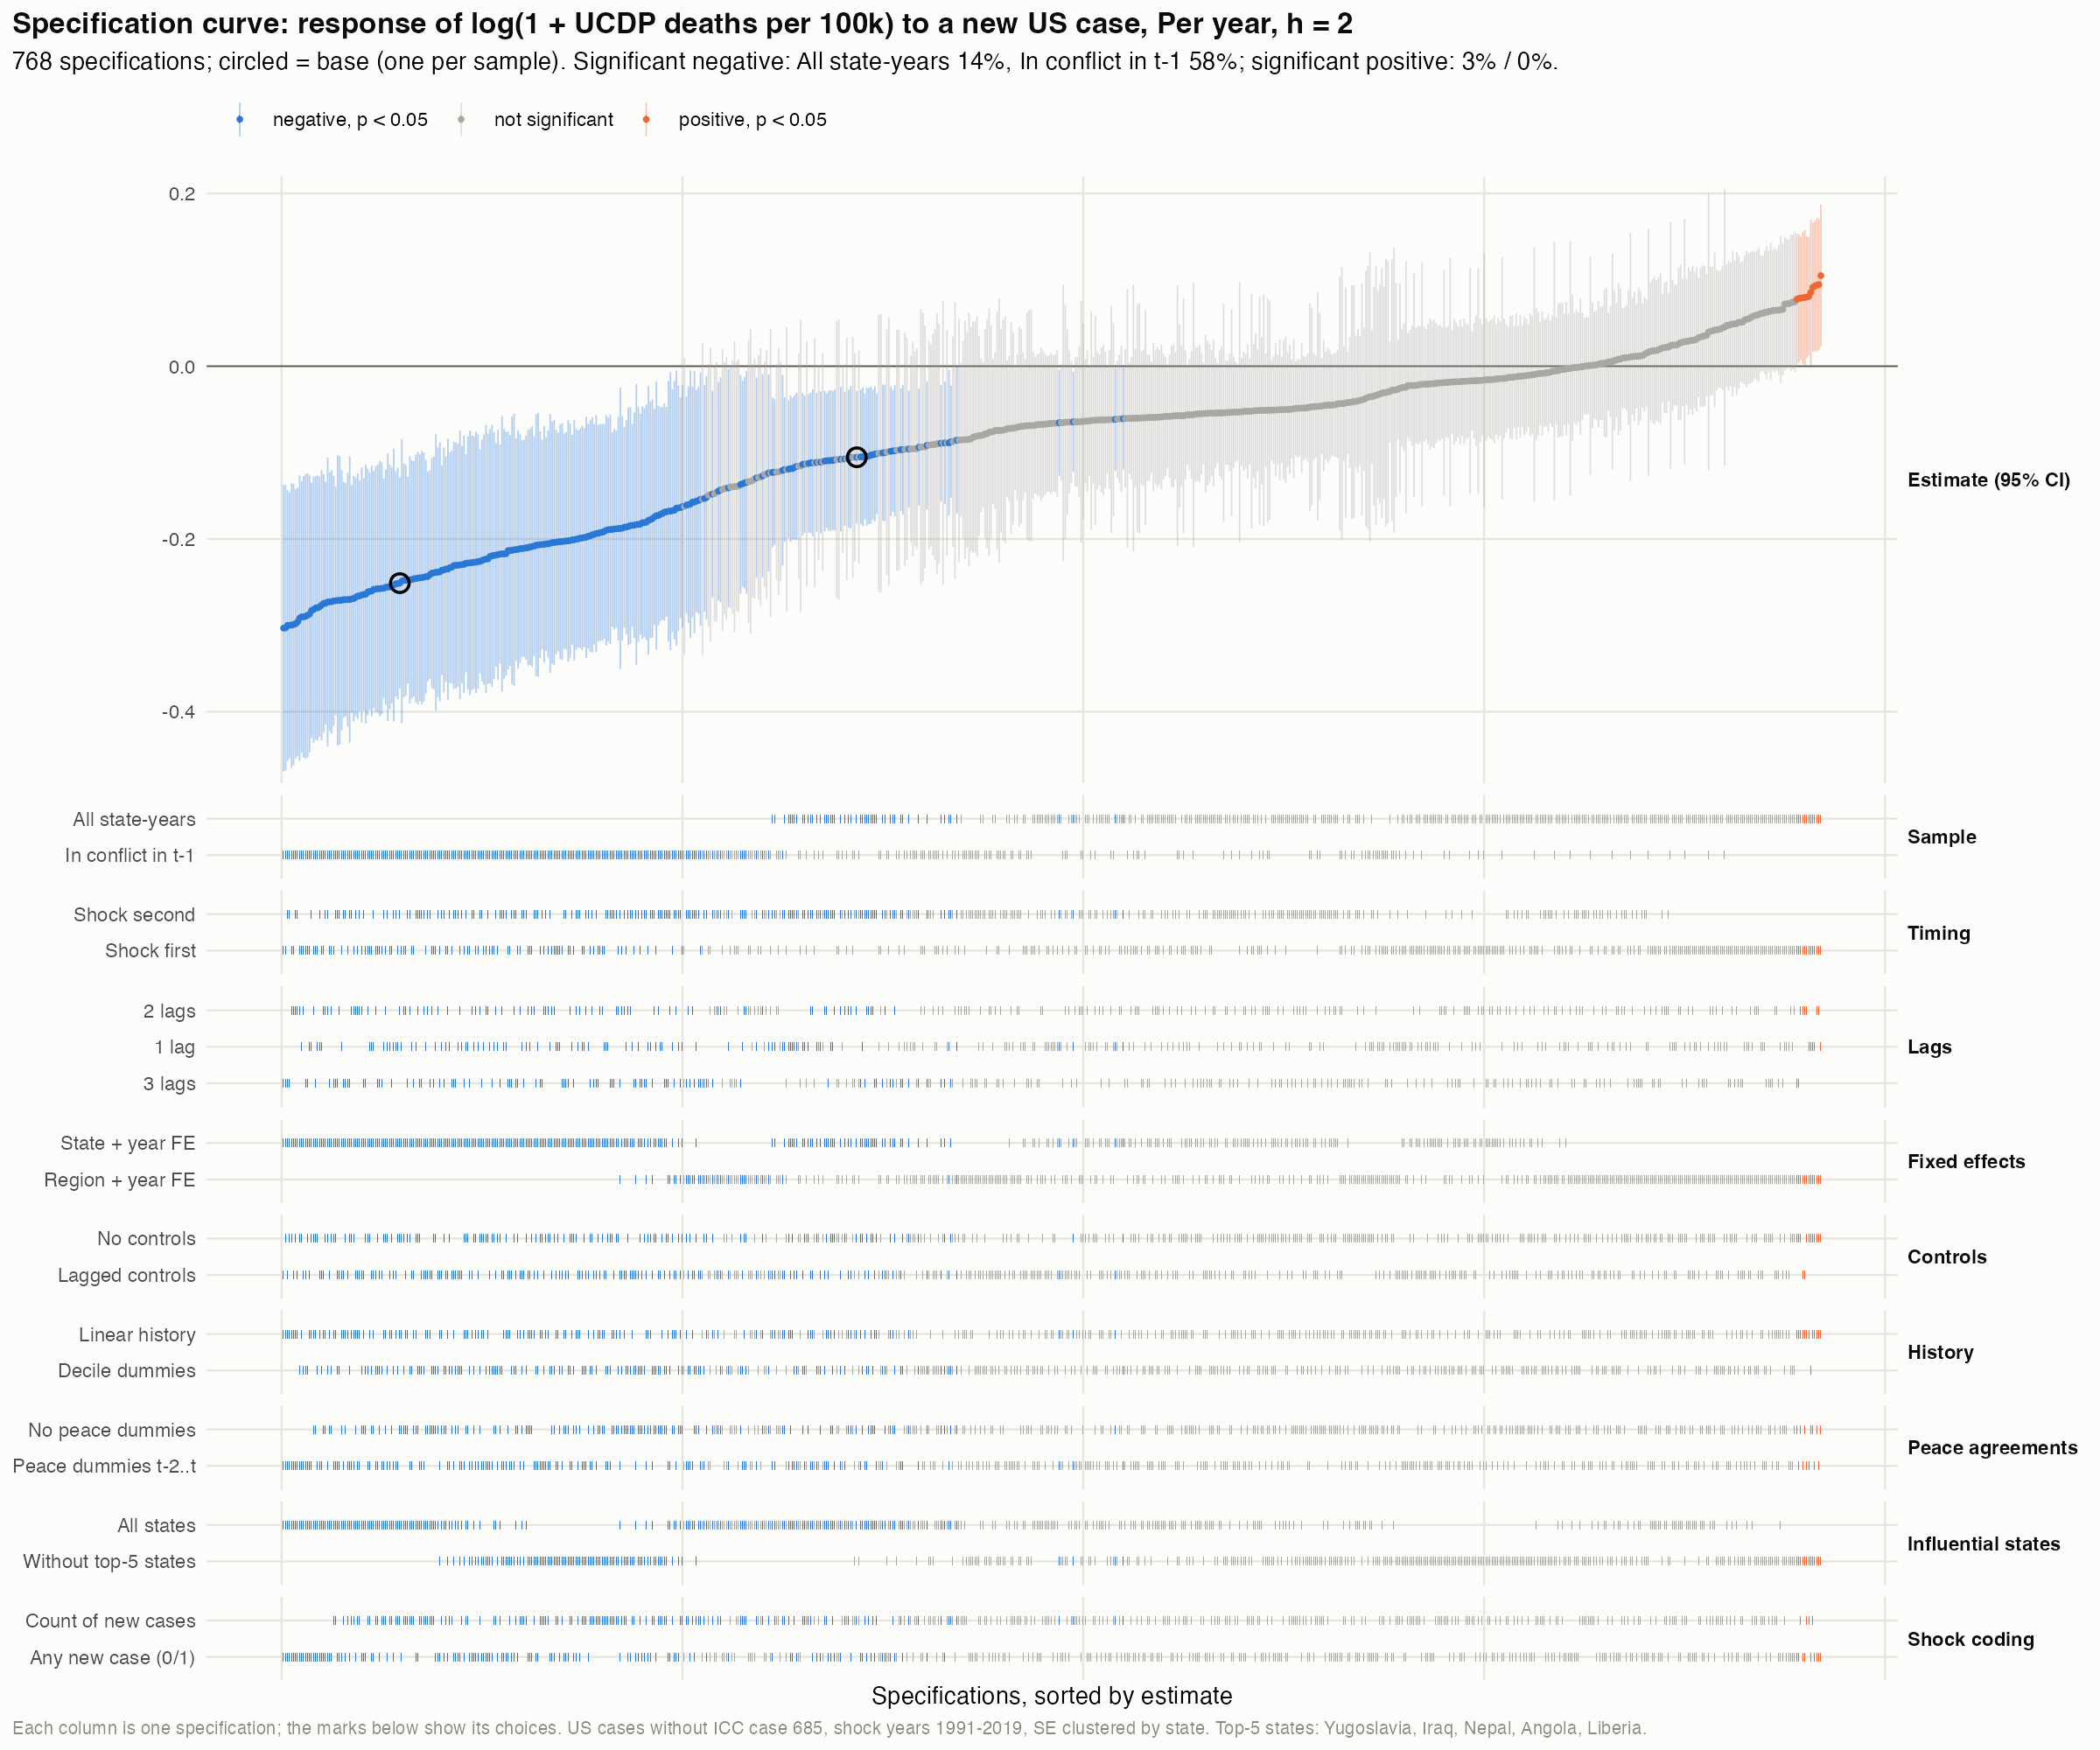
\includegraphics[width=0.85\textwidth]{fig39_us_spec_curve_h2.png}
\caption{Specification curve, $h=2$. Each column is one specification; the marks below show its choices. Circled: base.}
\label{fig:curve}
\end{figure}

\begin{table}[H]
\centering\small
\caption{Where the result holds, $h=2$}
\begin{tabular}{@{}lccc@{}}
\toprule
& Specifications & Median & Significantly negative \\
\midrule
In conflict, state + year FE & 192 & $-0.23$ & 100\,\% \\
In conflict, region + year FE & 192 & $-0.09$ & 16\,\% \\
All state-years, state FE, base timing, all states & 48 & $-0.11$ & 100\,\% \\
All state-years, state FE, other timing or top-5 dropped & 144 & about $-0.04$ & 0--8\,\% \\
All state-years, region + year FE & 192 & $+0.01$ & 1\,\% \\
\bottomrule
\end{tabular}
\end{table}

The decisive choice is country vs.\ region fixed effects. With region effects sanctioned countries are compared
mostly with \emph{other} countries, and the countries the US sanctions are persistently more violent; country fixed
effects compare a country with itself, which is the design's point. Region effects are therefore a weaker design, not
an equally valid alternative, but the curve shows openly that the result rests on the within-country comparison.

\section{Matched difference-in-differences}
\label{sec:matching}

As an alternative to regression adjustment, each US sanction-year is compared with three state-years \emph{of the same
year} without a new US case in $t-2..t+3$, with the same conflict status in $t-1$ and the same recent US cases, nearest
by Mahalanobis distance on deaths in $t$, $t-1$, $t-2$, the sanction stock, a US sanction in force, and democracy (with
replacement; caliper of 0.5 SD on deaths in $t$). The outcome is the change in deaths since the sanction year, so the
same-year comparison plays the role of year effects and the differencing that of country effects. The effect is the
mean over treated events (ATT); a bias-adjusted version regresses it on the remaining covariate gaps
\citep{abadieimbens2011}. 72 of 104 US events in wars are matched (149 of 216 overall). Most unmatched events follow another new US case in
the two preceding years: a clean control cannot have one, so the exact match drops them; the estimand is therefore the
effect of a new US sanction \emph{after at least two years without one}. Deaths in $t-3$ and $t-4$, which
were not matched on, are balanced (standardised differences 0.05 and 0.00); sanction history and democracy remain
somewhat imbalanced, hence the adjustment.

\begin{figure}[H]
\centering
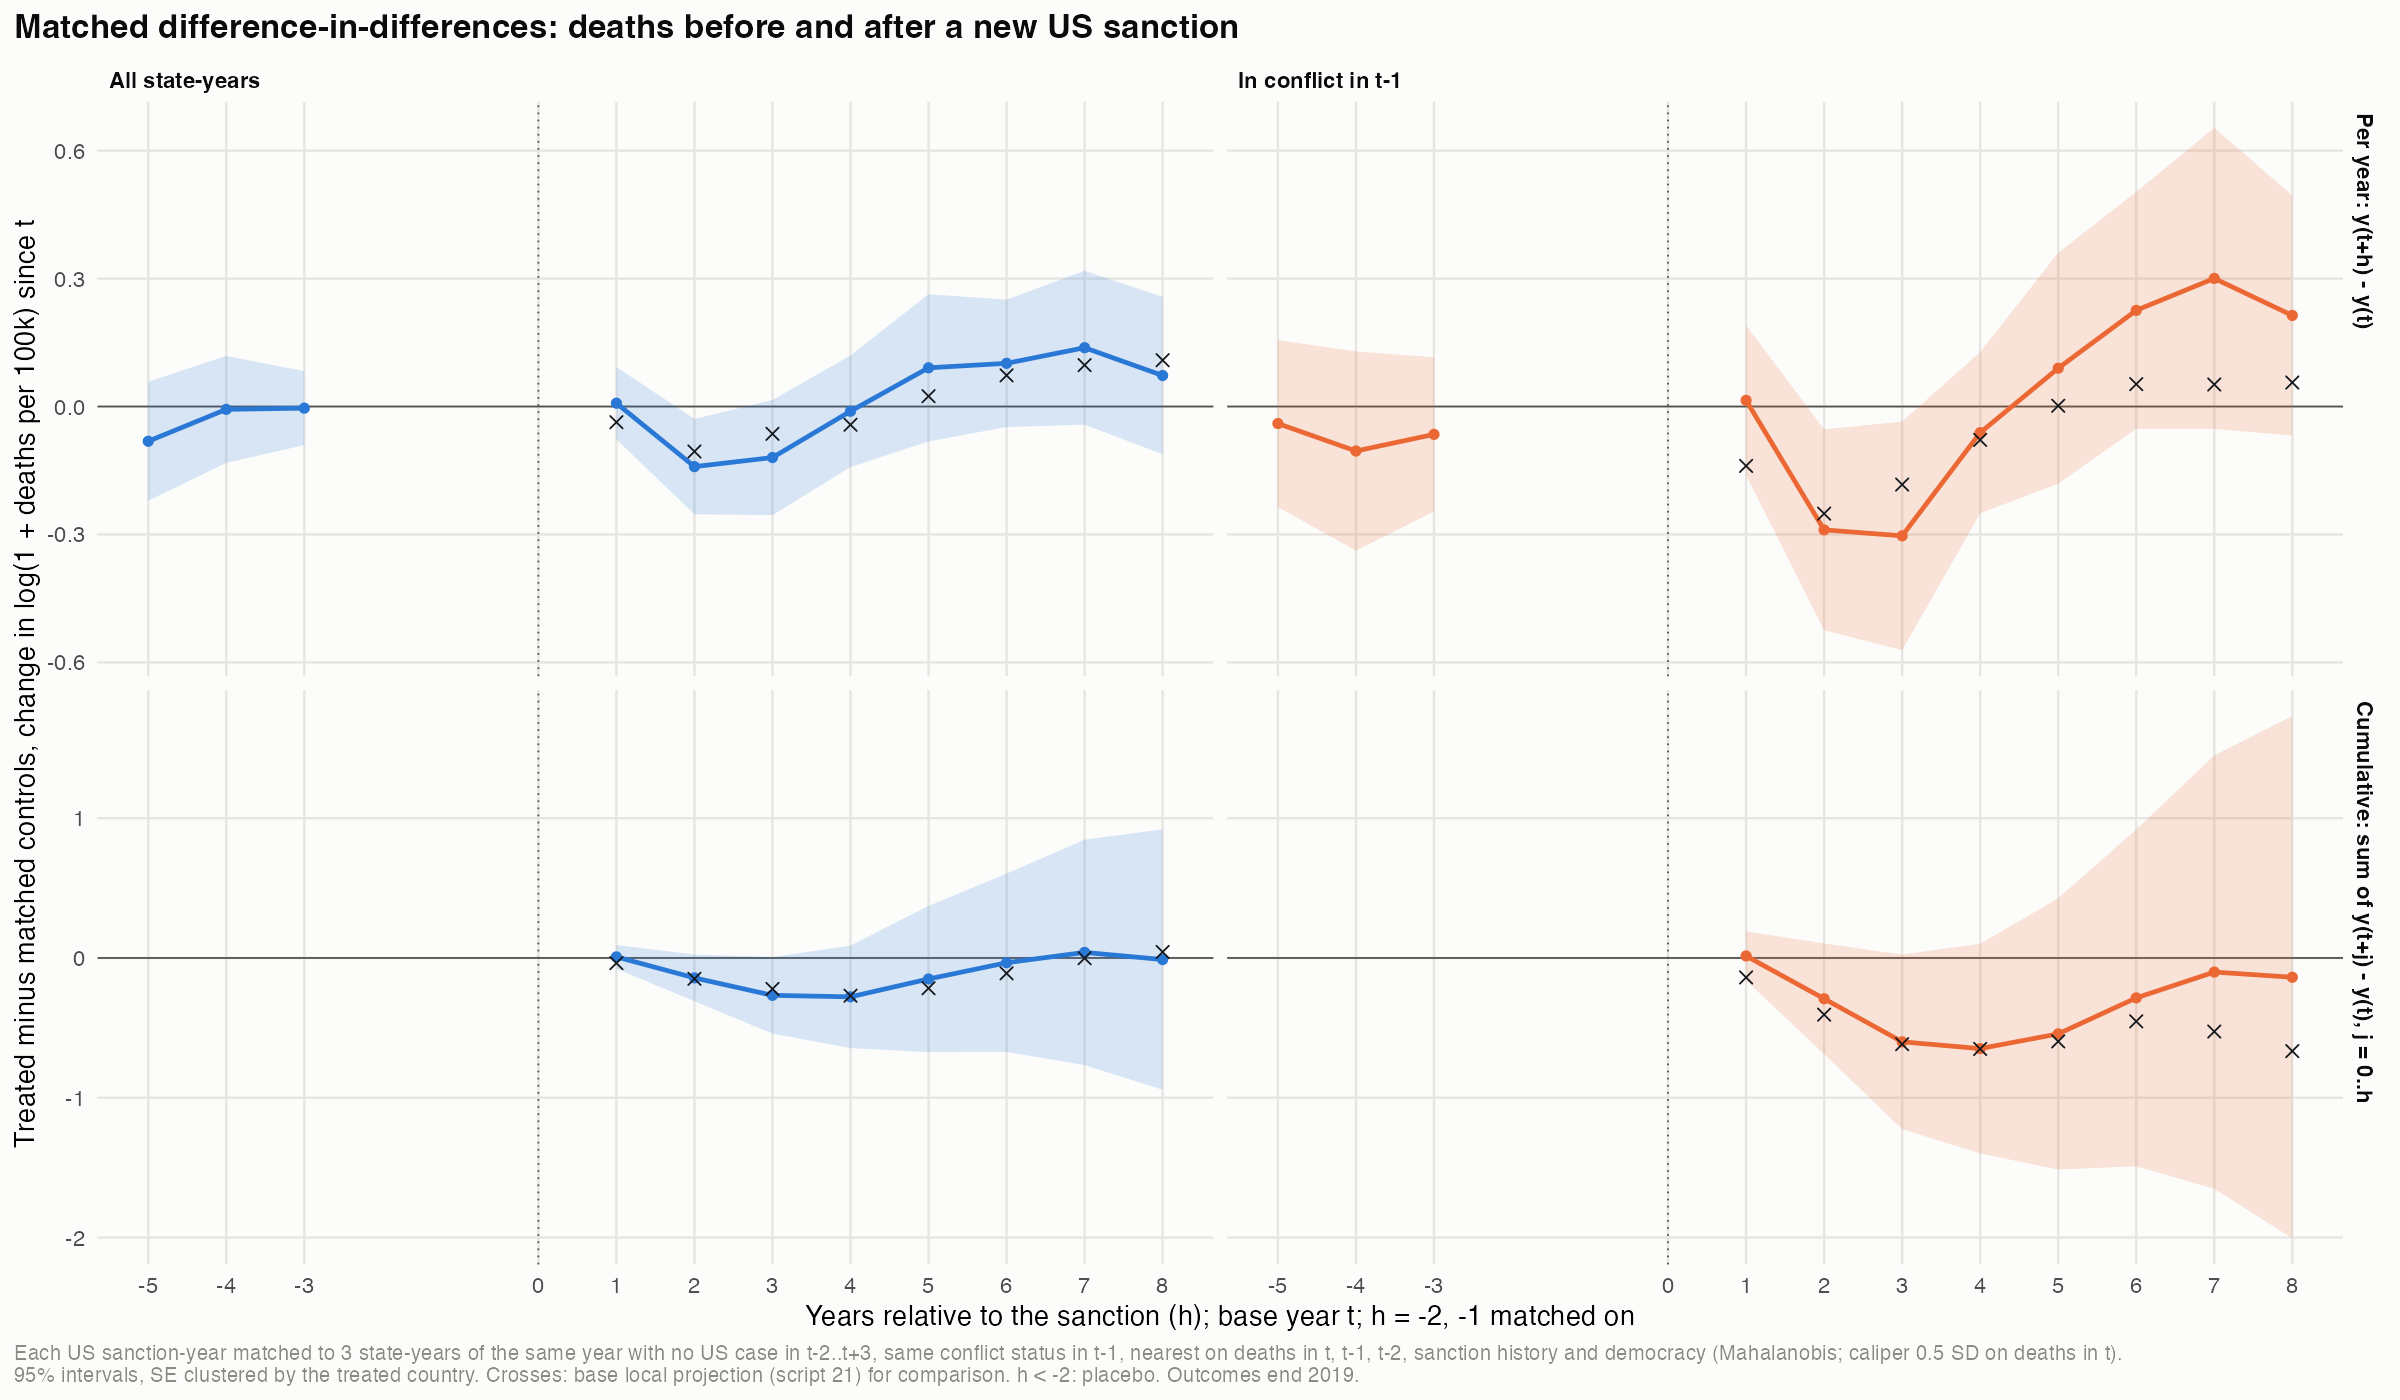
\includegraphics[width=0.95\textwidth]{fig40_us_matching_path.png}
\caption{Matched difference-in-differences. Crosses: the base local projection for comparison.}
\label{fig:matchpath}
\end{figure}

\begin{figure}[H]
\centering
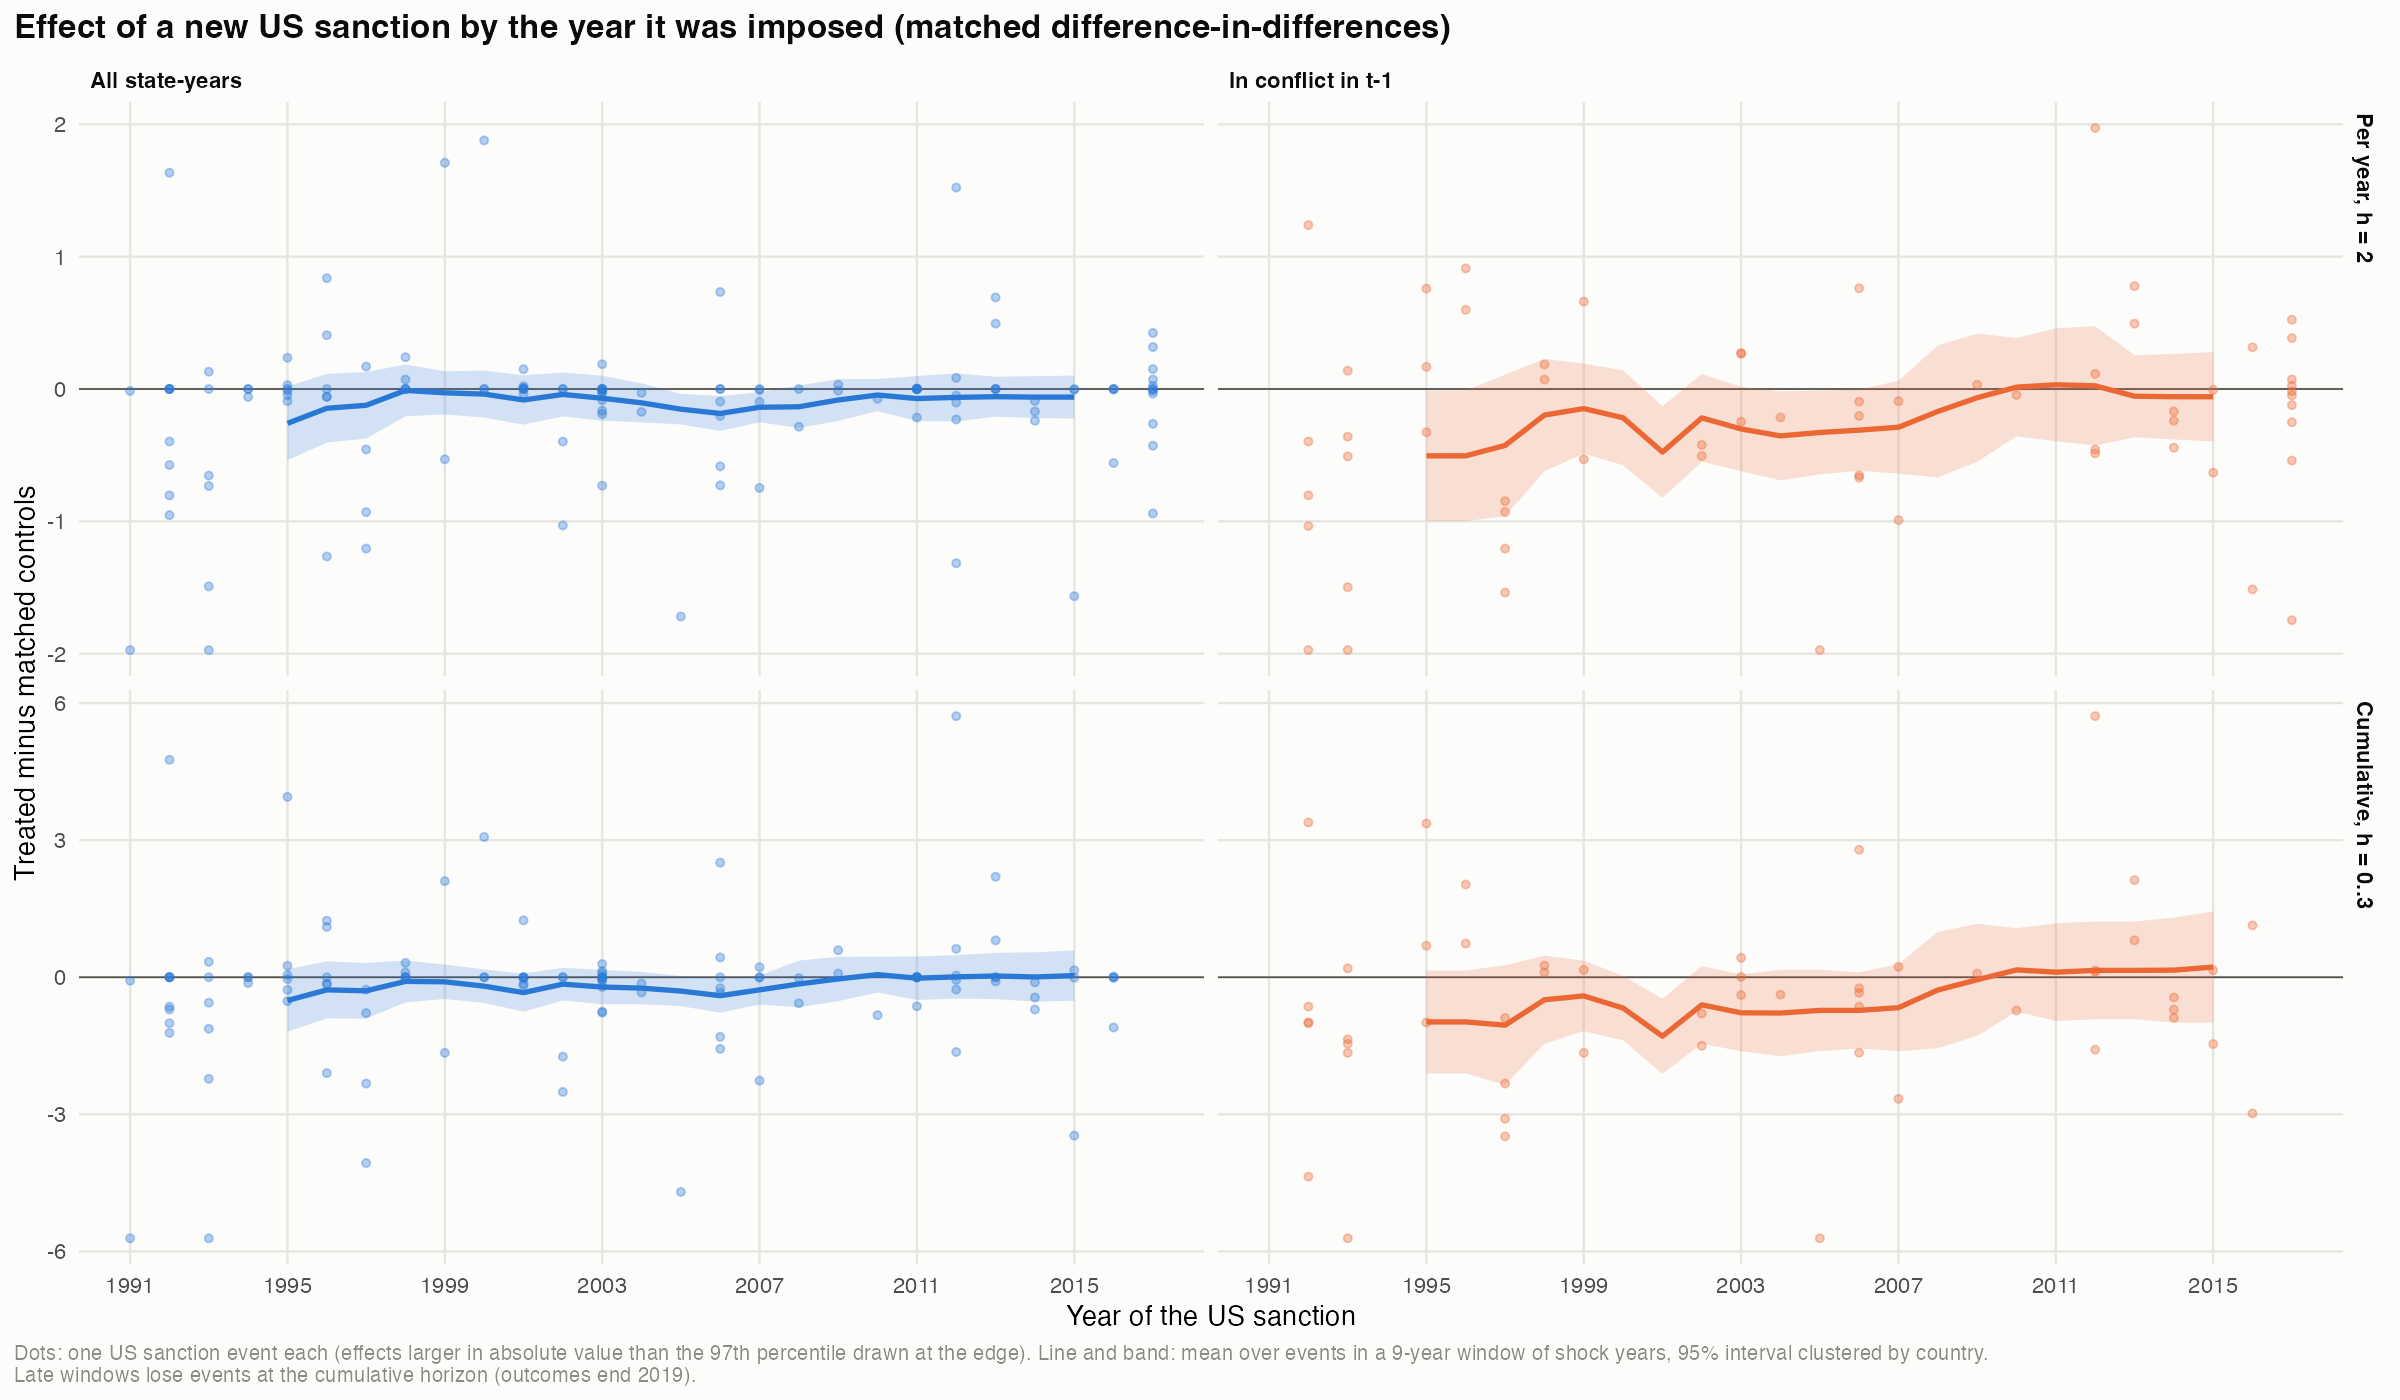
\includegraphics[width=0.95\textwidth]{fig41_us_matching_over_time.png}
\caption{Matched effect by the year of the sanction. Dots: single events; line: nine-year rolling mean with 95\,\% interval.}
\label{fig:matchtime}
\end{figure}

\begin{table}[H]
\centering\small
\caption{Matched effect by period of the sanction, $h=2$ [events]}
\begin{tabular}{@{}lccc@{}}
\toprule
& 1991--99 & 2000--09 & 2010--19 \\
\midrule
In conflict in $t-1$ & $-0.51$\sig{*} [23] & $-0.33$\sig{*} [15] & $-0.06$ [24] \\
All state-years & $-0.26$\sig{*} [43] & $-0.10$ [44] & $-0.06$ [41] \\
\bottomrule
\end{tabular}
\end{table}

The matching design reproduces the dip with a different identification: no pre-trend, $-0.29$\sig{**} at $h=2$ and
$-0.30$\sig{**} at $h=3$ in wars ($-0.43$\sig{**} bias-adjusted). It differs from the local projection in two ways: the
dip is followed by a rebound at $h=6$--8 ($+0.2$ to $+0.3$, not significant), and within wars the effect declines
over the decades, from about $-0.5$ for 1990s sanctions to about zero for 2010s sanctions. With 14--25 events per
window none of the period differences is significant.

\section{Propensity-score matching and the matching estimand}
\label{sec:pscore}

The lecture's matching estimand,
$\beta_M = \int \big[E(Y_i\mid D_i=1,X_i=x) - E(Y_i\mid D_i=0,X_i=x)\big]\,dF_X(x)$, compares units with the same
characteristics and weights the differences by the distribution of $x$ among \emph{all} units (the ATE); with weights
$dF_{X\mid D=1}$ it is the effect on the sanctioned (ATT). Conditioning on the propensity score instead of $x$, I
estimate both: a logit of a new US case (clean events as above) on deaths in $t$, $t-1$, $t-2$, sanction history,
democracy, region and period (AUC 0.74); nearest-neighbour matching on its logit within the same year in both
directions \citep{abadieimbens2006}, without and with the conventional caliper of 0.2 SD; and subclassification on five
score blocks, which writes the integral as a weighted sum. Overlap is good (73 of 76 war events on common support).

\begin{table}[H]
\centering\small
\caption{Propensity-score matching, $h=2$ (bootstrap SE)}
\begin{tabular}{@{}lccc@{}}
\toprule
& ATE (lecture estimand) & ATT & ATC \\
\midrule
In conflict, nearest neighbour & $-0.12$ (0.12) & $-0.11$ (0.19) & $-0.12$ (0.12) \\
In conflict, caliper 0.2 SD & $-0.25$ (0.25) & $-0.27$ (0.28) & $-0.25$ (0.25) \\
In conflict, subclassification & $-0.02$ (0.16) & $-0.07$ (0.13) & $-0.02$ (0.16) \\
All state-years, nearest neighbour & $-0.21$\sig{**} (0.08) & $-0.10$ (0.10) & $-0.21$\sig{**} (0.08) \\
All state-years, subclassification & $-0.04$ (0.05) & $-0.07$ (0.08) & $-0.04$ (0.05) \\
\bottomrule
\end{tabular}
\end{table}

Every estimate among wars is negative but none is significant; with the standard caliper the ATT ($-0.27$) equals the
covariate-matching ATT, without it or by subclassification it is close to zero. Matching on a single score leaves
pairs that differ in violence levels, which drive the outcome path; covariate matching on violence directly is more
precise. The ATE is not the natural target here: it weights by all units, mostly unsanctioned state-years, and in all
state-years the significant ATE comes entirely from imputing sanction effects for peaceful, democratic states the US
rarely sanctions (poor balance, 0.47 SD) --- extrapolation. The policy-relevant estimand is the ATT.

\begin{figure}[H]
\centering
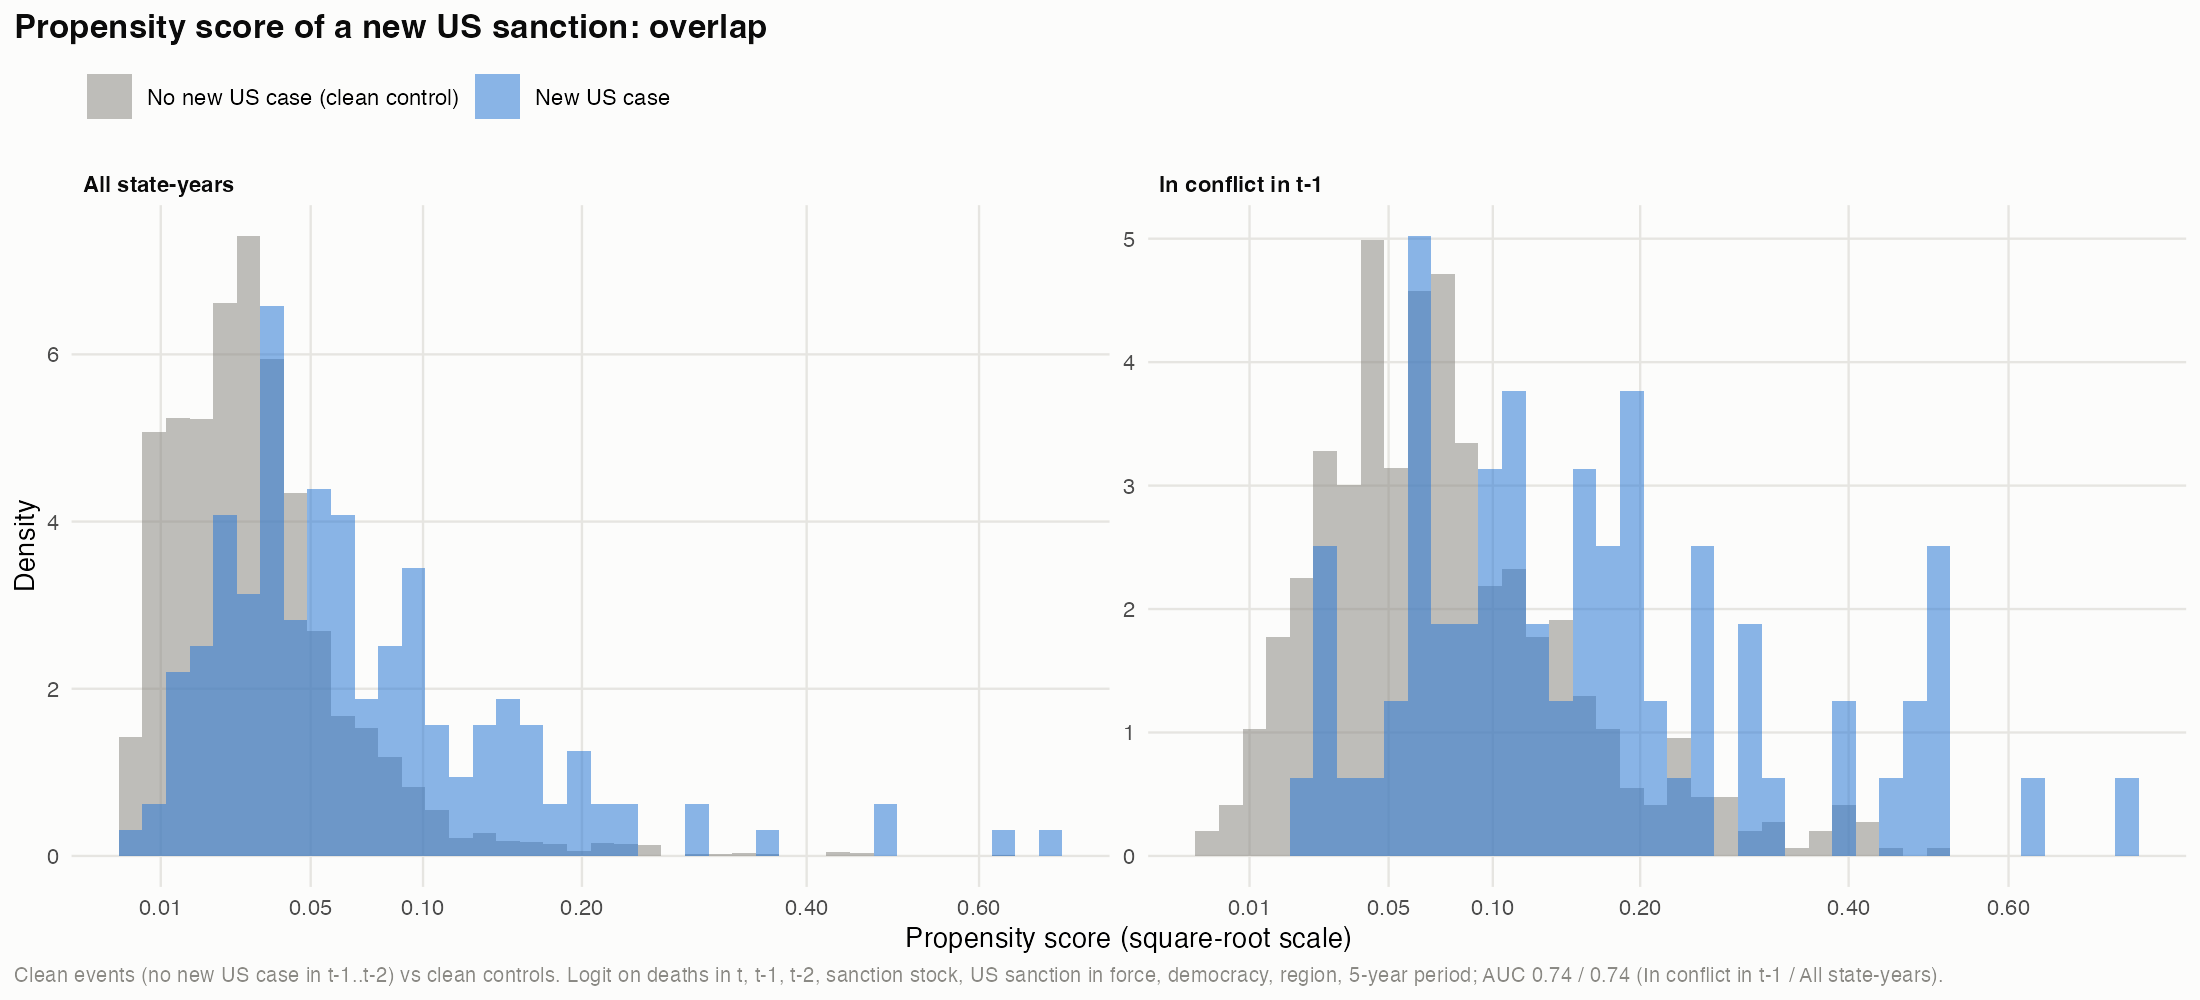
\includegraphics[width=0.75\textwidth]{fig42_us_pscore_overlap.png}
\caption{Propensity score of a new US sanction (clean events) and of clean controls.}
\end{figure}

% =============================================================================
\parttitle{Part C --- Added 17.11.2026: matching on violence, other senders, LP-DiD with the authors' code}
% =============================================================================

\section{Who is compared with whom, and matching on the score and on violence}
\label{sec:who}

Propensity-score matching compares units with the same \emph{score}, not the same situation. Listing the pairs
(Figure~\ref{fig:who}, left) shows the problem: in wars, the correlation between a sanctioned event's deaths in $t$ and
its matched controls' deaths is only 0.29. Pakistan 1993 (0.04 log deaths per 100k) is matched to Sierra Leone,
Tajikistan and Djibouti (2.55 on average); Indonesia 1992 (0.03) to Somalia, Lebanon and Djibouti (2.98). In 2017 Somalia,
Sudan, Egypt and Eritrea share the same three controls (Thailand, Afghanistan, Jordan). Balance holds on average,
not pair by pair, and the outcome is a change since $t$, which depends on the level.

A new version therefore matches on both: controls of the same year within 0.2 SD of the score's logit \emph{and}
within 0.5 SD of deaths in $t$ (the caliper of the covariate matching), nearest on the standardised distance in both
(Figure~\ref{fig:who}, right). Pairs now look alike (deaths in $t$, $t-1$, $t-2$ within $\pm0.06$ SD), but only 34 of
63 war events find such a control. The ones that do not are the most violent (Angola 1993, Iraq 1997, Somalia 2010,
Afghanistan 1999/2011) and those with the highest scores (the Middle East 2016--18, Iran 2012): no unsanctioned
country in that year looks like them. The ATT is $-0.22$ (0.27) in wars and $-0.10$ (0.07) overall --- between the
score-only ($-0.11$) and the covariate matching ($-0.29$), not significant.

\begin{figure}[H]
\centering
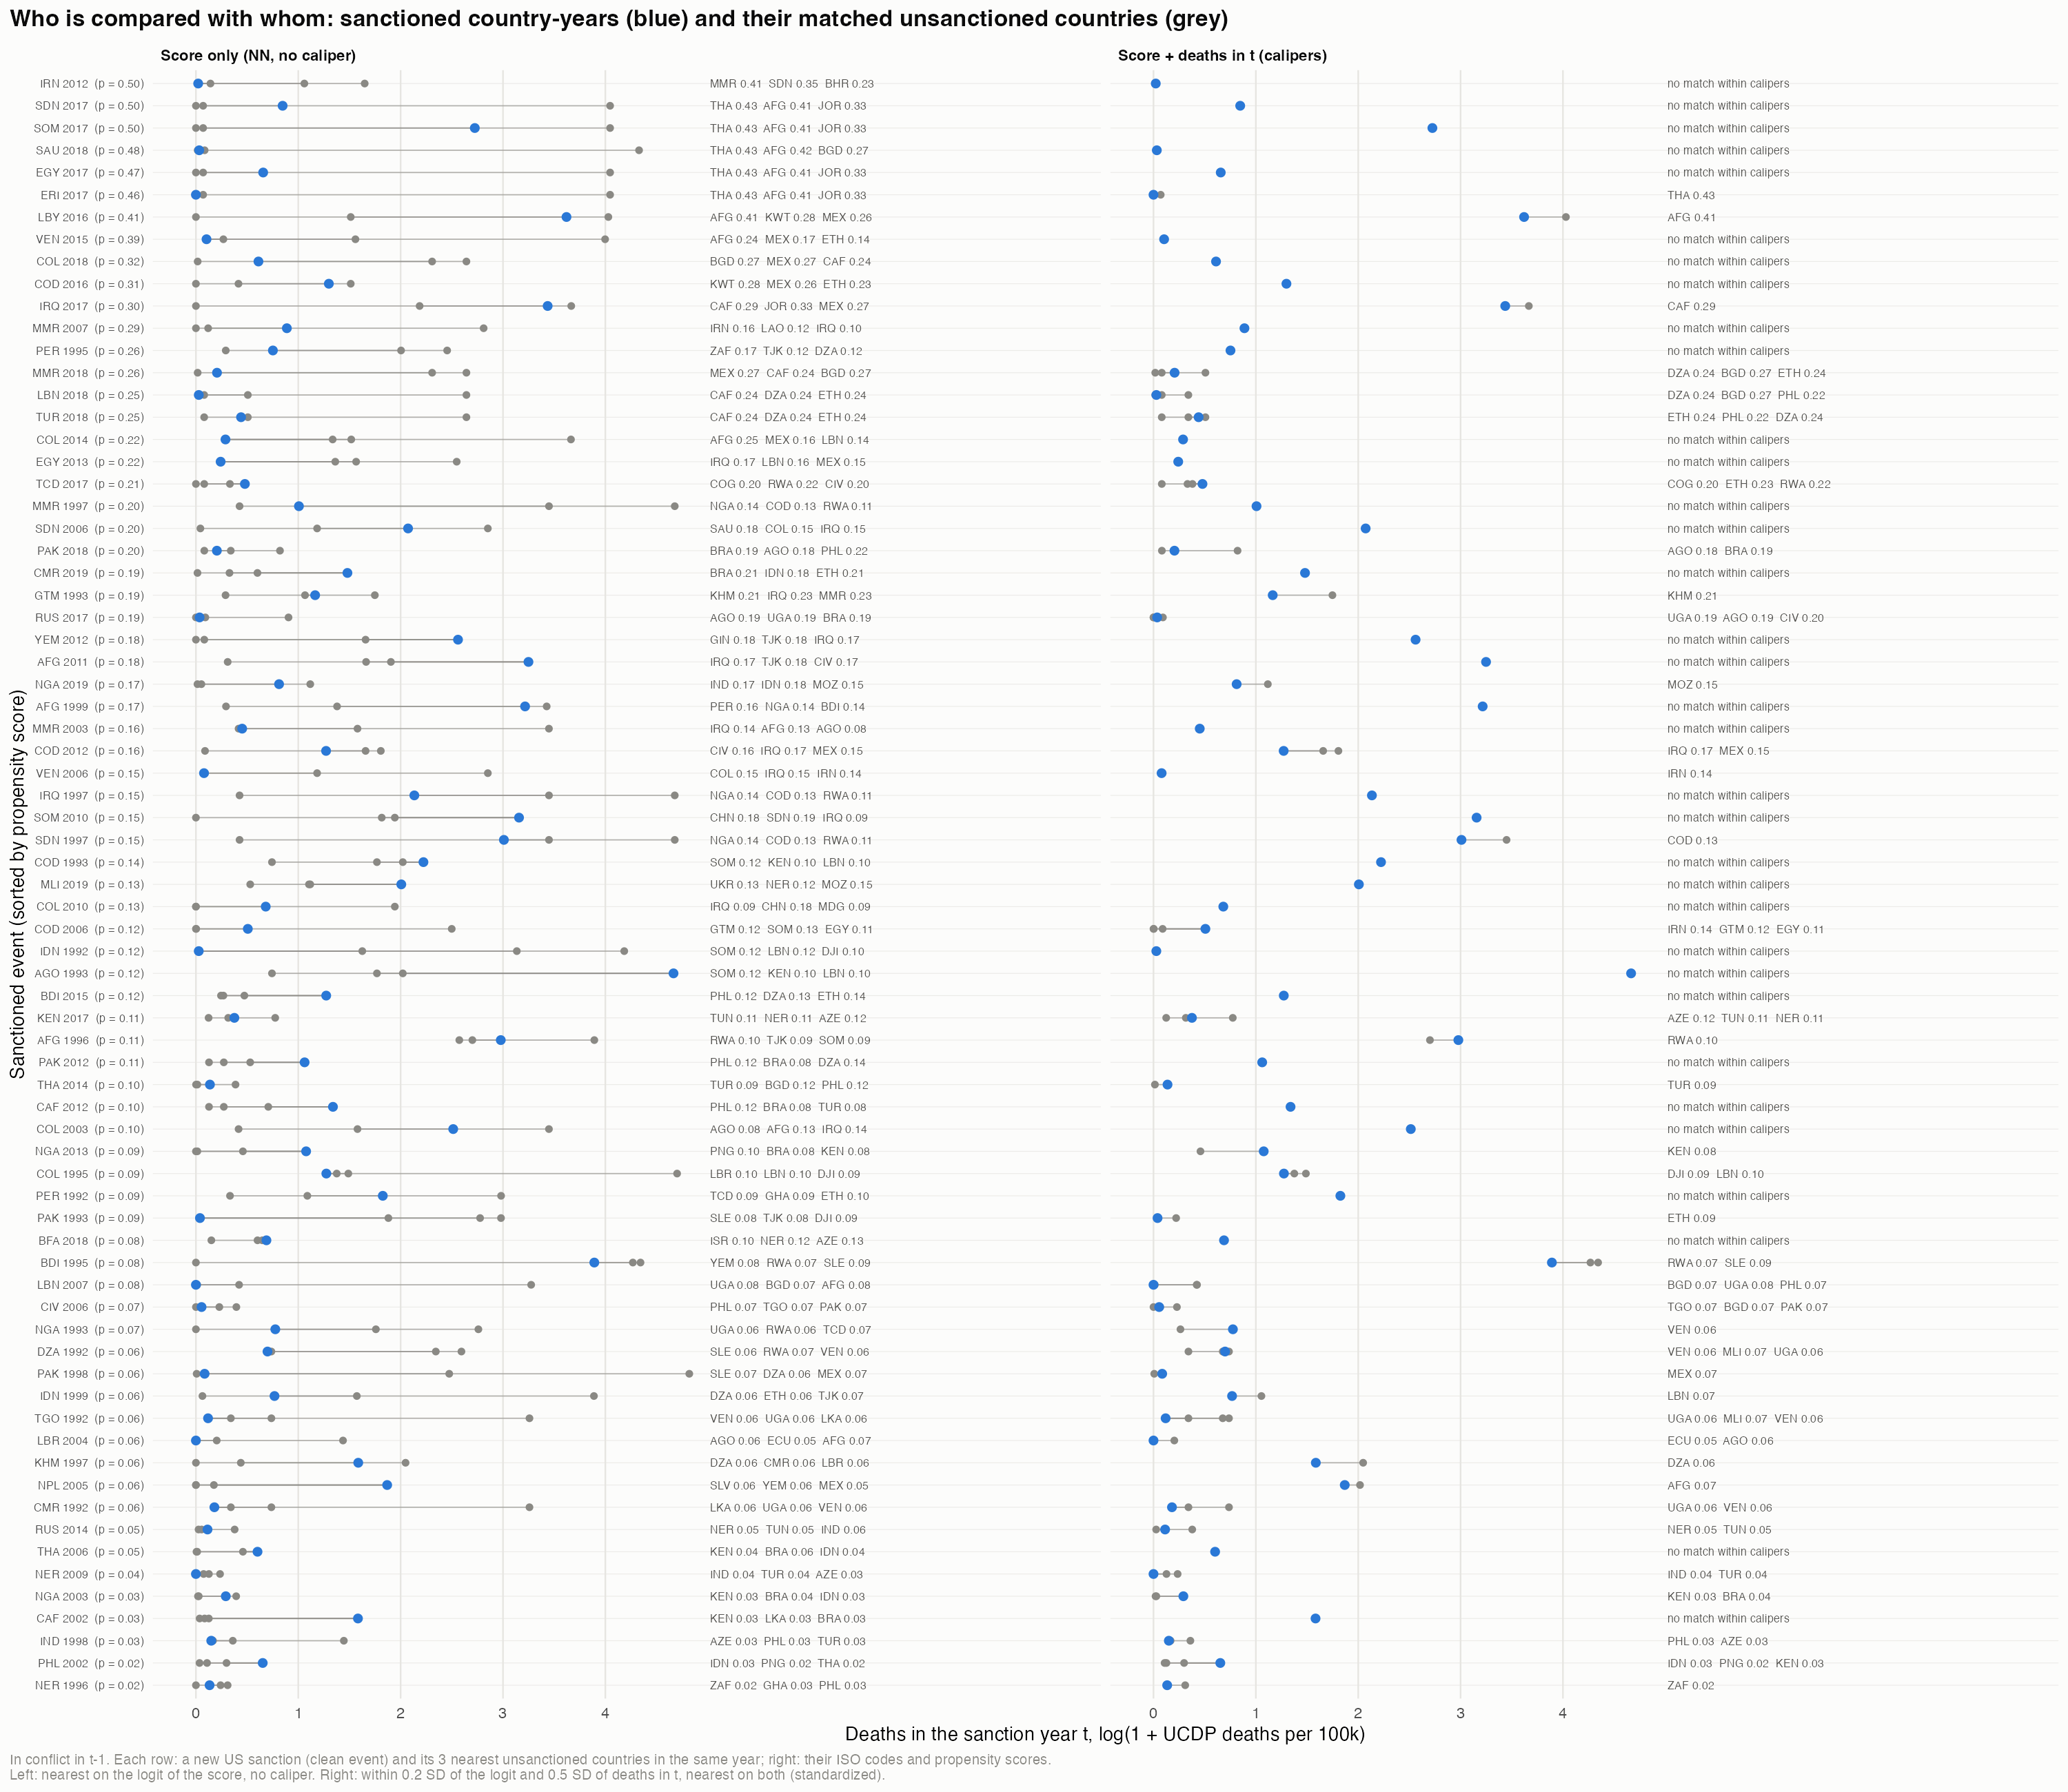
\includegraphics[width=\textwidth]{fig44_us_pscore_who_matches_whom.png}
\caption{Who is compared with whom (wars). Each row: a sanctioned event (blue, deaths in $t$) and its matched
unsanctioned countries of the same year (grey), with their ISO codes and scores. Left: score only. Right: score and
deaths in $t$.}
\label{fig:who}
\end{figure}

\section{Sanctions by sender: any, US, UN, Western rich}
\label{sec:senders}

The US measure is almost purely unilateral: in 1991--2019, 242 of 245 new US cases have the US as the only sender, and
none is a UN case (UN cases have ``UN'' as the sender; only 17 US case-targets fall in a year with a new UN case). I
re-ran every design with three other shocks: any sender (835 cases), UN (71), and Western rich --- every sender a
Western rich state or the EU, UN cases excluded (522; this includes the US cases and drops EU cases joined by
non-rich countries such as Albania, Serbia or Ukraine). Controls are clean for the same group.

\begin{table}[H]
\centering\small
\caption{Effect at $h=2$ by sender, in conflict in $t-1$}
\label{tab:senders}
\begin{threeparttable}
\begin{tabular}{@{}lcccc@{}}
\toprule
& Any sender & United States & UN & Western rich \\
\midrule
Local projection (D11), per case & $-0.070$\sig{***} & $-0.251$\sig{***} & $-0.100$ & $-0.111$\sig{***} \\
Matched DiD, covariates (ATT) & $+0.122$ & $-0.289$\sig{**} & $+0.451$ & $-0.110$ \\
PS matching, nearest neighbour (ATT) & $+0.039$ & $-0.109$ & $-0.223$ & $-0.041$ \\
PS matching, score + deaths (ATT) & $-0.036$ & $-0.224$ & $+0.502$ & $+0.009$ \\
Shock years / events (LP) & 187 & 85 & 49 & 132 \\
\bottomrule
\end{tabular}
\begin{tablenotes}\footnotesize
\item Standard errors in \texttt{empirics/results/tables/sender\_comparison.md}. The LP coefficient is per new case,
the matching estimates per event, so compare signs across senders, not sizes across designs. Western rich without the
US cases, LP: $-0.110$\sig{**} (0.042) in wars, $-0.042$ (0.035) overall.
\end{tablenotes}
\end{threeparttable}
\end{table}

The US is the only sender negative in every design and the only one a matching design confirms. In the local
projection, however, the decline is not only a US phenomenon (Table~\ref{tab:senderlp}, Figure~\ref{fig:senderlp}):
\begin{itemize}[leftmargin=*]
\item \textbf{At $h=2$} the US effect is the largest ($-0.25$ in wars); Western rich senders give about half of it
  ($-0.11$\sig{***}), and the same without the US cases, so that part is not the US. Any sender together is smaller
  still ($-0.07$\sig{***}): the many other senders dilute the US and Western effects.
\item \textbf{UN sanctions have a different shape:} smaller and insignificant in any single year ($-0.10$ at $h=2$), but
  the decline persists and cumulates, to $-0.89$\sig{*} by $h=5$ and $-1.84$\sig{**} by $h=8$ in wars, while the US dip
  closes by $h=5$. There is no pre-trend ($h=-5..-3$: all $p\ge0.26$).
\item \textbf{Caveats:} the UN result rests on 71 cases in 28 countries, concentrated in a few wars (Liberia 7, Iran 6,
  Iraq 5, Afghanistan 5, Sudan 4); whether it survives dropping single countries is not checked. Matching cannot
  confirm it: UN cases target the most violent wars, where comparable unsanctioned countries are scarce (7--30 matched
  events, estimates from $-0.39$ to $+0.50$). For Western rich senders matching puts the effect near zero.
\end{itemize}

\begin{table}[H]
\centering\small
\caption{Local projection (D11) by sender: effect of one new case on $\log(1+\text{deaths per 100k})$}
\label{tab:senderlp}
\begin{threeparttable}
\begin{tabular}{@{}lcccc@{}}
\toprule
& Any sender & United States & UN & Western rich \\
\midrule
\multicolumn{5}{@{}l}{\emph{In conflict in $t-1$}} \\
$h=2$ & $-0.070$\sig{***} (0.024) & $-0.251$\sig{***} (0.062) & $-0.100$ (0.093) & $-0.111$\sig{***} (0.029) \\
Cumulative $0..3$ & $-0.180$\sig{***} (0.052) & $-0.617$\sig{***} (0.140) & $-0.507$\sig{*} (0.277) & $-0.252$\sig{***} (0.066) \\
Cumulative $0..5$ & $-0.220$\sig{**} (0.086) & $-0.597$\sig{**} (0.291) & $-0.893$\sig{*} (0.451) & $-0.252$\sig{**} (0.112) \\
Cumulative $0..8$ & $-0.299$ (0.191) & $-0.666$ (0.560) & $-1.836$\sig{**} (0.793) & $-0.250$ (0.224) \\
Shock-years & 187 & 85 & 49 & 132 \\
\addlinespace
\multicolumn{5}{@{}l}{\emph{All state-years}} \\
$h=2$ & $-0.026$ (0.020) & $-0.105$\sig{***} (0.039) & $-0.162$ (0.132) & $-0.045$\sig{*} (0.025) \\
Cumulative $0..3$ & $-0.049$ (0.046) & $-0.222$\sig{***} (0.079) & $-0.523$\sig{*} (0.311) & $-0.081$ (0.059) \\
Cumulative $0..5$ & $-0.028$ (0.077) & $-0.217$ (0.156) & $-1.051$\sig{**} (0.491) & $-0.042$ (0.101) \\
Cumulative $0..8$ & $+0.059$ (0.148) & $+0.043$ (0.338) & $-1.428$\sig{***} (0.549) & $+0.105$ (0.176) \\
Shock-years & 459 & 183 & 64 & 291 \\
\bottomrule
\end{tabular}
\begin{tablenotes}\footnotesize
\item Base specification (D11) with the shock replaced by the number of new cases of each group. Standard errors
clustered by state. Western rich without the US cases: $h=2$ $-0.110$\sig{**} (0.042) in wars, $-0.042$ (0.035) overall.
\end{tablenotes}
\end{threeparttable}
\end{table}

\begin{figure}[H]
\centering
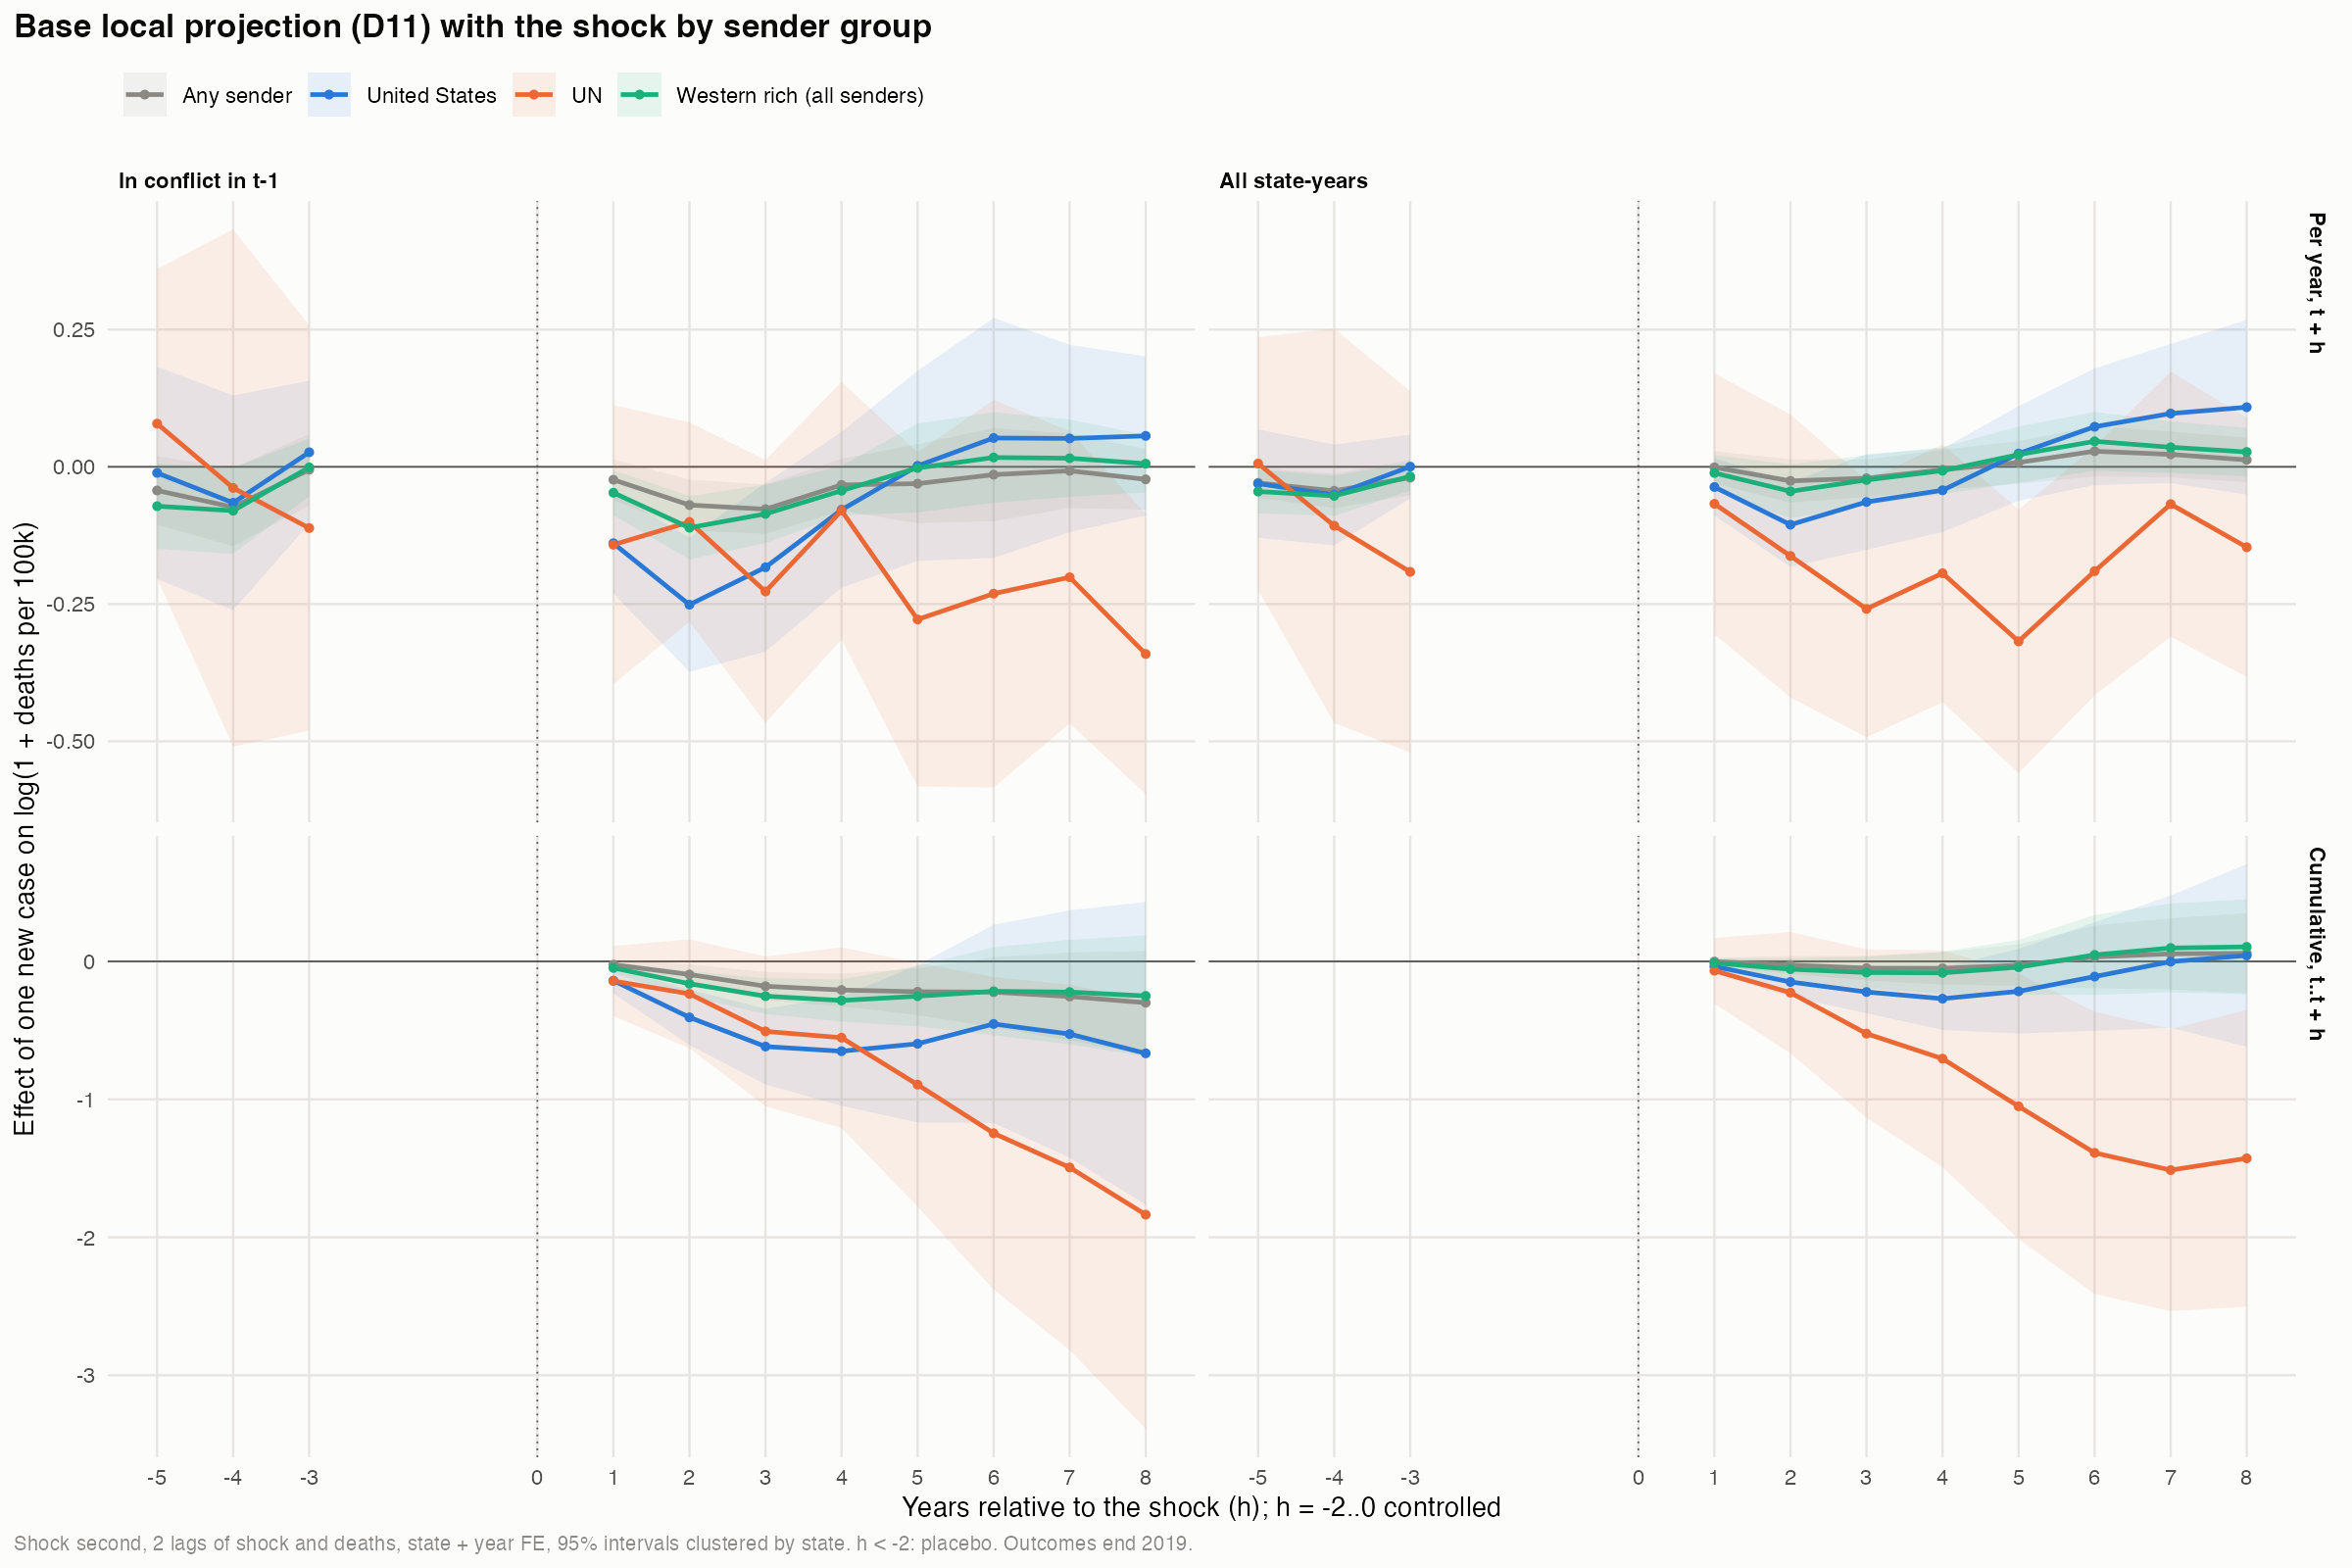
\includegraphics[width=0.95\textwidth]{fig46_sender_lp_paths.png}
\caption{Local projection (D11) by sender: per-year and cumulative paths, both samples (95\,\% intervals).
$h=-2..0$ are controlled for and therefore not estimated.}
\label{fig:senderlp}
\end{figure}

\begin{figure}[H]
\centering
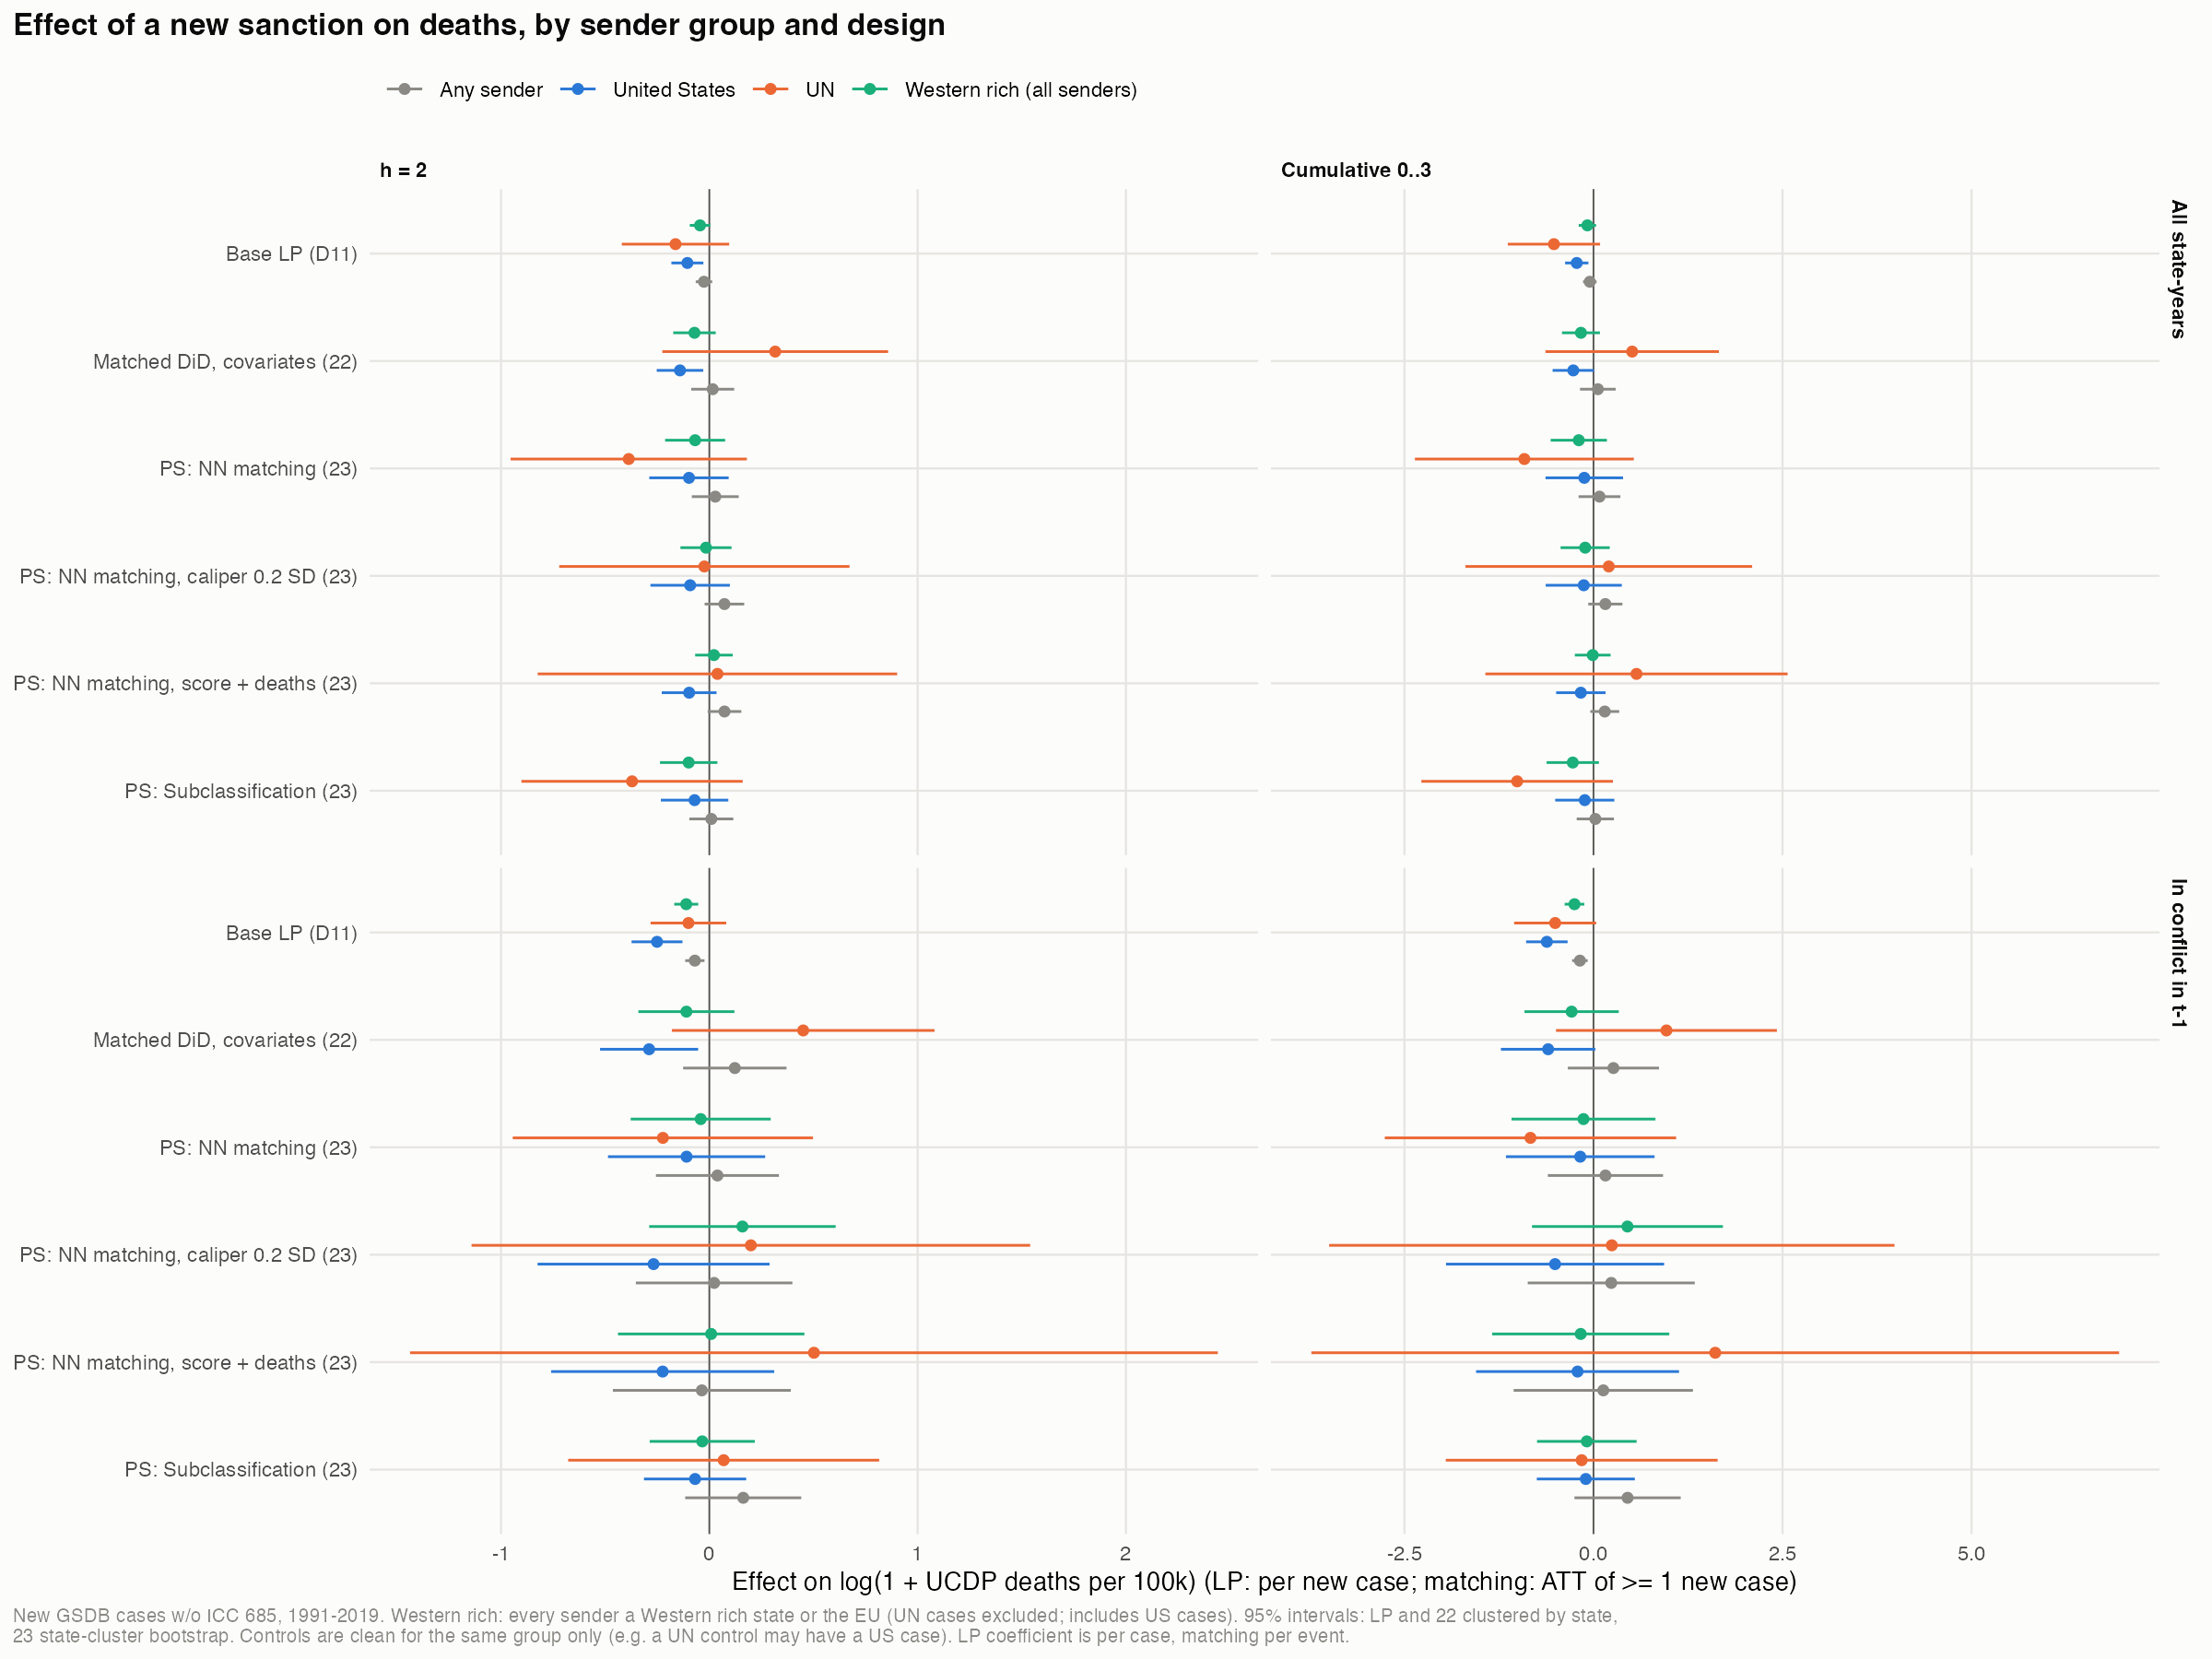
\includegraphics[width=0.9\textwidth]{fig45_sender_comparison.png}
\caption{Effect at $h=2$ and cumulated over 0--3 by sender and design, both samples (95\,\% intervals).}
\label{fig:senders}
\end{figure}

\section{LP-DiD with the authors' code}
\label{sec:lpdid}

The earlier LP-DiD (October) was our own implementation and used any sender. This one follows the authors' published
reference code \citep{dube2025}: the R examples for the estimation (long difference $y_{t+h}-y_{t-1}$ on a 0/1
treatment with year effects, standard errors clustered by state, variance-weighted and reweighted to equal weights per
event), and their Stata example for non-absorbing treatment for the clean-control windows, since a country can be
sanctioned repeatedly. A sanctioned country counts if it had no new US case in the three years before $t$ and none in
$t+1..t+h$; a control has none in $t-3..t+h$. Unlike the base specification, the reference year is $t-1$ and past
deaths are not controlled for. I report two outcomes, log deaths and conflict incidence (0/1).

\begin{figure}[H]
\centering
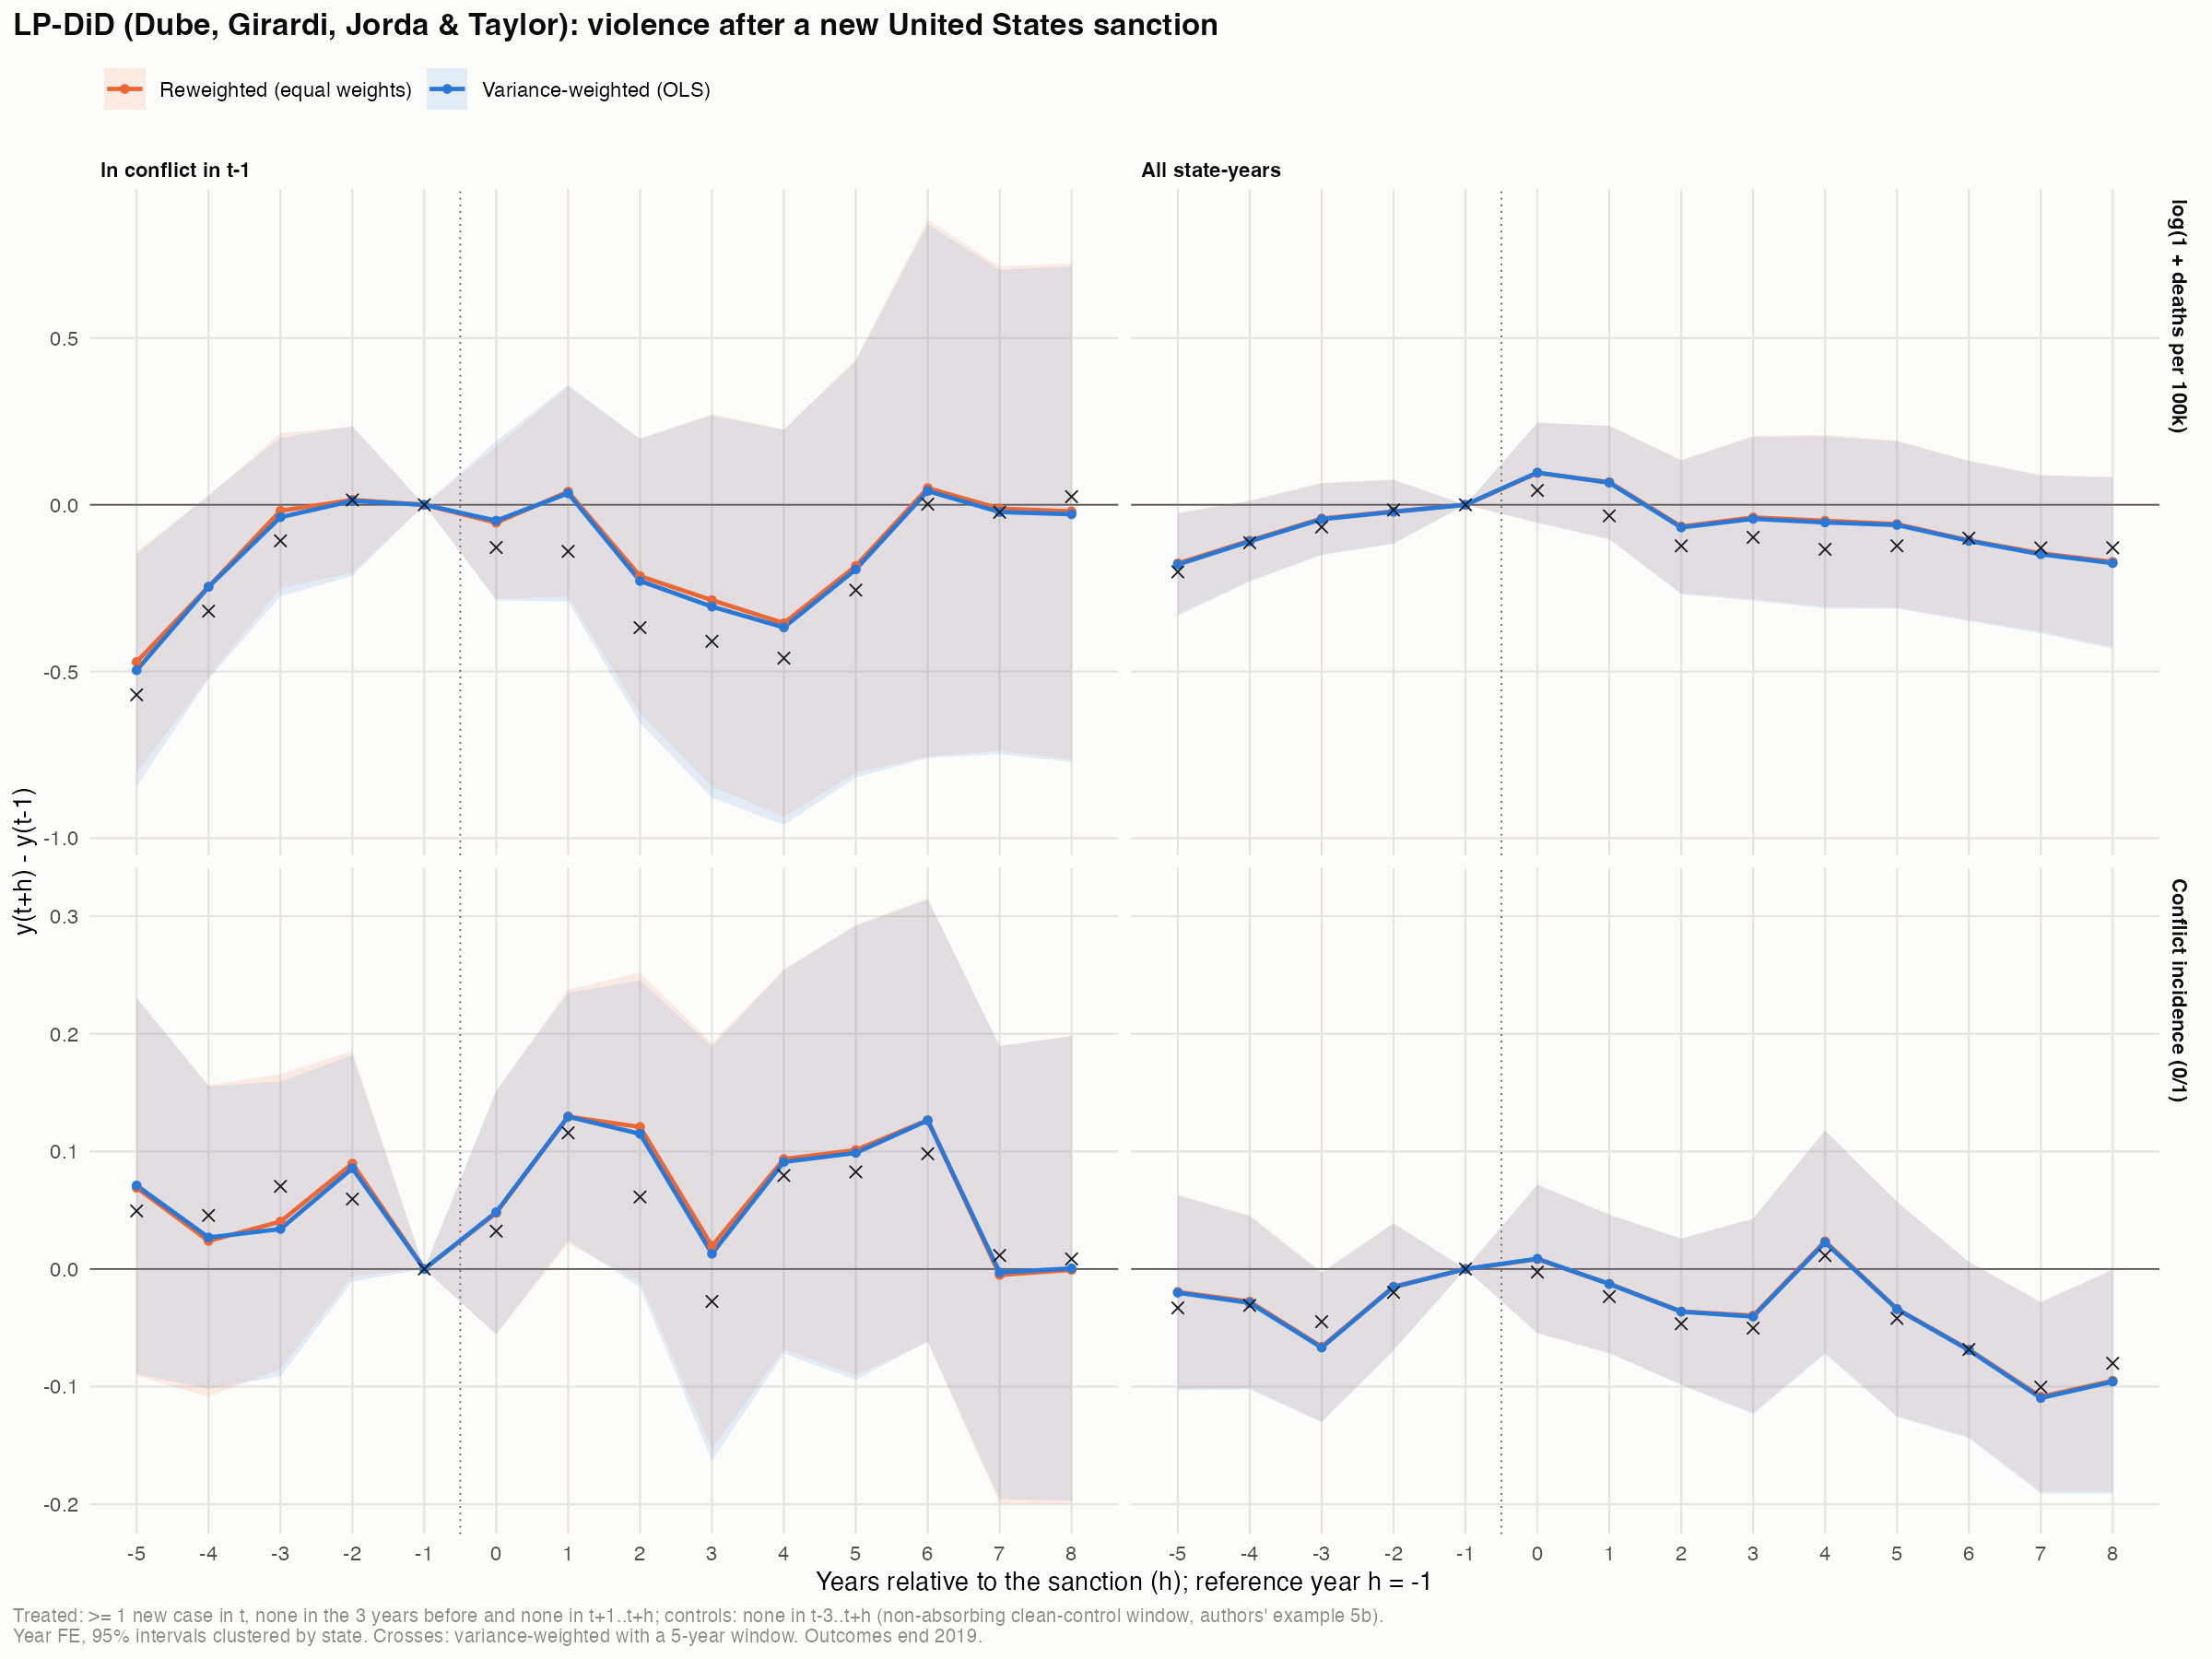
\includegraphics[width=0.95\textwidth]{fig47_lpdid_dgjt.png}
\caption{LP-DiD for new US sanctions. Top: log deaths; bottom: conflict incidence. Bands: 95\,\% intervals of the
3-year window (variance-weighted and reweighted overlap); crosses: 5-year window.}
\label{fig:lpdid}
\end{figure}

\begin{table}[H]
\centering\small
\caption{LP-DiD, in conflict in $t-1$, variance-weighted, 3-year window}
\label{tab:lpdid}
\begin{threeparttable}
\begin{tabular}{@{}lccccccc@{}}
\toprule
$h$ & $-5$ & $-4$ & $-2$ & 0 & 1 & 2 & 4 \\
\midrule
Log deaths & $-0.50$\sig{***} & $-0.25$\sig{*} & $0.01$ & $-0.05$ & $0.03$ & $-0.23$ & $-0.37$ \\
& (0.18) & (0.14) & (0.12) & (0.12) & (0.17) & (0.22) & (0.30) \\
Conflict incidence & $0.07$ & $0.03$ & $0.09$\sig{*} & $0.05$ & $0.13$\sig{**} & $0.12$\sig{*} & $0.09$ \\
& (0.08) & (0.07) & (0.05) & (0.05) & (0.05) & (0.07) & (0.08) \\
Sanctioned events & 38 & 45 & 64 & 75 & 59 & 46 & 30 \\
\bottomrule
\end{tabular}
\begin{tablenotes}\footnotesize
\item Reference year $h=-1$. Stars: \sig{*}~$p<0.1$, \sig{**}~$p<0.05$, \sig{***}~$p<0.01$; at the 5\,\% level
(the figure's bands) only deaths at $h=-5$ and incidence at $h=1$ differ from zero. Equal weights give the same
numbers to two decimals; the 5-year window gives $-0.37$ to $-0.41$ for deaths at $h=2..4$.
\end{tablenotes}
\end{threeparttable}
\end{table}

\begin{itemize}[leftmargin=*]
\item \textbf{Before the sanction:} in wars, deaths five years earlier were 0.5 log points lower relative to the
  controls ($p<0.01$); $h=-4$ is significant only at 10\,\%, and the last two years before the sanction are parallel.
  The US sanctions wars that escalated three to five years earlier and have since stayed high. The base
  specification holds deaths in $t$, $t-1$, $t-2$ fixed, which covers the plateau but not the earlier escalation.
\item \textbf{After:} a dip of $-0.23$ to $-0.37$ at $h=2..4$, the same shape as the local projection, not
  significant; back to zero by $h=6$. Requiring no further US case through $t+h$ leaves 46 events at $h=2$.
\item \textbf{Incidence:} wars are not more likely to end after a US sanction; at $h=1$ they continue more often
  ($+13$ pp, $p<0.05$). Fewer deaths in wars that go on, in line with the termination result in
  Section~\ref{sec:peace}.
\end{itemize}

\section{Where this leaves the project}
\label{sec:final}

\begin{itemize}[leftmargin=*]
\item \textbf{Consistent:} for US sanctions on countries at war, every design --- local projection, doubly robust
  weighting, covariate matching, propensity-score matching in four versions, LP-DiD --- gives a negative estimate two
  to four years after the sanction, of $-0.07$ to $-0.4$ log points, fading by $h=5$--6 (the panel VAR, estimated
  on all state-years only, agrees there).
  It is clearest for the US. In the local projection Western rich senders (also without the US) and UN sanctions
  are followed by fewer deaths too --- for the UN smaller per year but cumulating over eight years --- but matching
  supports only the US effect, and the UN result rests on a few wars.
\item \textbf{Significant only with adjustment for past violence:} the local projection, doubly robust weighting
  and covariate matching on violence. Designs that need a comparable unsanctioned country in the same year keep
  30--75 events and lose significance.
\item \textbf{Not identified:} the US sanctions wars after an escalation, and at the same time as wars are at a high
  level. With annual data, a post-sanction decline cannot be separated from wars that would have come down anyway.
  Selection on observables is the assumption throughout, and the LP-DiD's pre-period shows it is not innocuous.
\item \textbf{Not found:} that sanctions end wars, that the US effect lasts, or a robust effect outside wars.
\end{itemize}

\bibliographystyle{plainnat}
\bibliography{../../references,../2026-11-09/report_refs,report_refs}

\end{document}
